\documentclass{article}
\usepackage{graphicx} % Required for inserting images
\usepackage{amsmath}
\usepackage{geometry}
\usepackage{amssymb}
\usepackage{color}
\usepackage{CJKutf8}
\usepackage{float}
\usepackage{subfigure}
\usepackage{listings}
\usepackage{placeins}
\usepackage{enumitem}
\usepackage{booktabs}

\geometry{a4paper, scale=0.8}   
\linespread{2}
\definecolor{dark_green}{RGB}{0,102,51}
\title{Lab3 - TCP}
\author{Jiaxi Zhang}
\date{\today}
\begin{document}
\maketitle
\begin{CJK*}{UTF8}{gbsn}
\section{At a first look at the captured trace}
\subsection{In tcpethereal-trace-1}
The IP address of the client computer is 192.168.1.102,
and the TCP port number used by the client computer is 1161.
The IP address of gaia.cs.umass.edu is 128.119.245.12, and the TCP port number used by the server is 80.
It can be seen in the following two figures.
\begin{figure}[H]
\centering
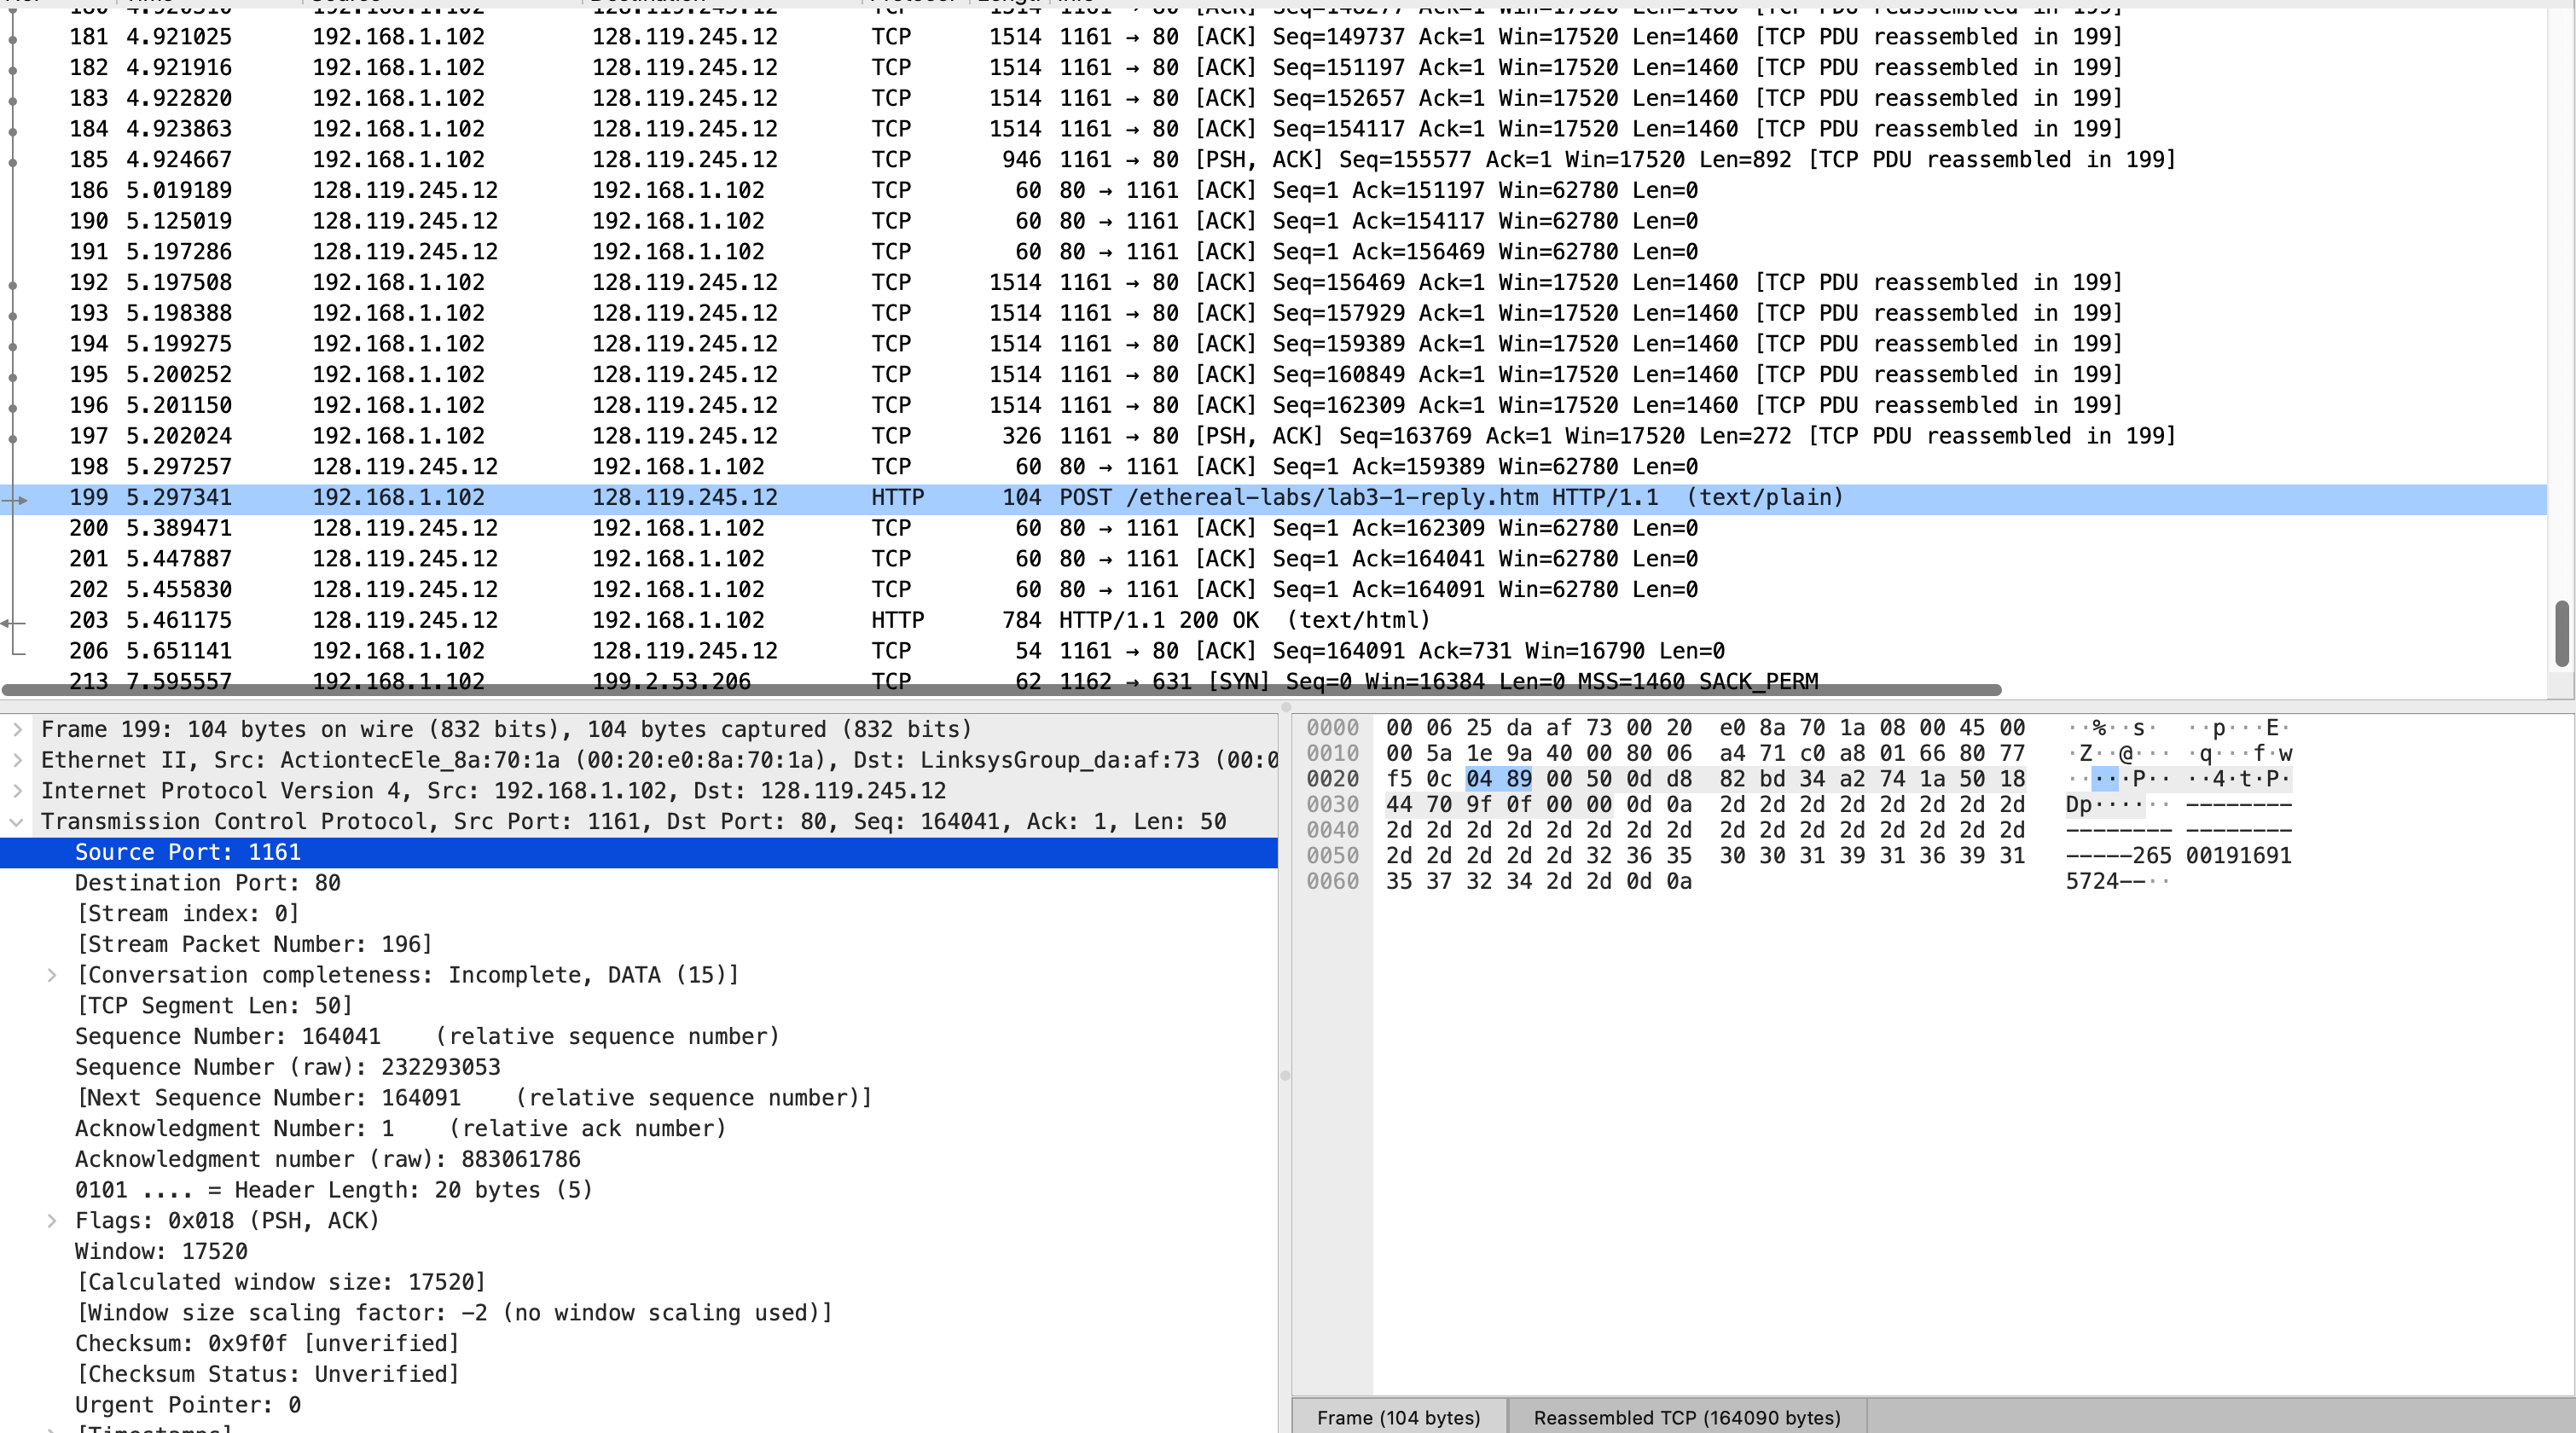
\includegraphics[width=0.8\textwidth]{1-2.png}
\end{figure}
\begin{figure}[H]
\centering
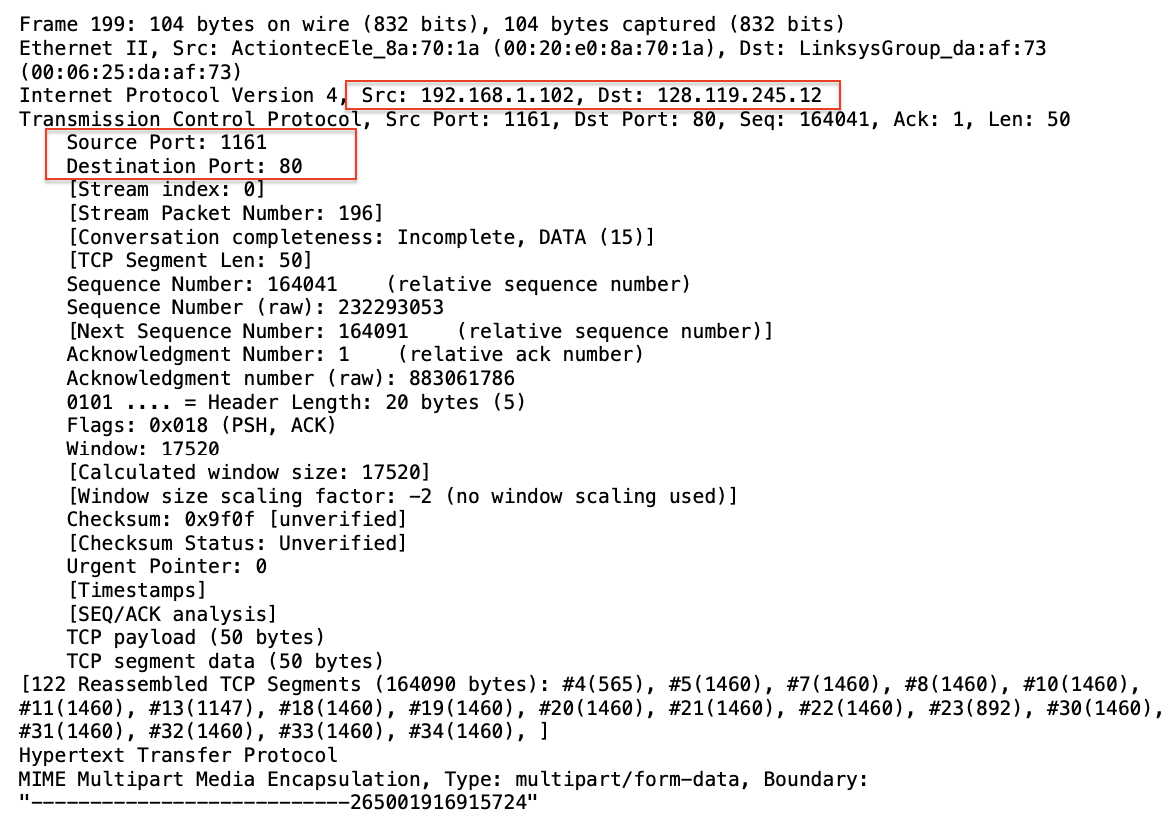
\includegraphics[width=0.8\textwidth]{1-1.png}
\end{figure}

\subsection{In my trace}
The IP address of the client computer is 10.17.204.99,
and the TCP port number used by the client computer is 64699.
\begin{figure}[H]
    \centering
    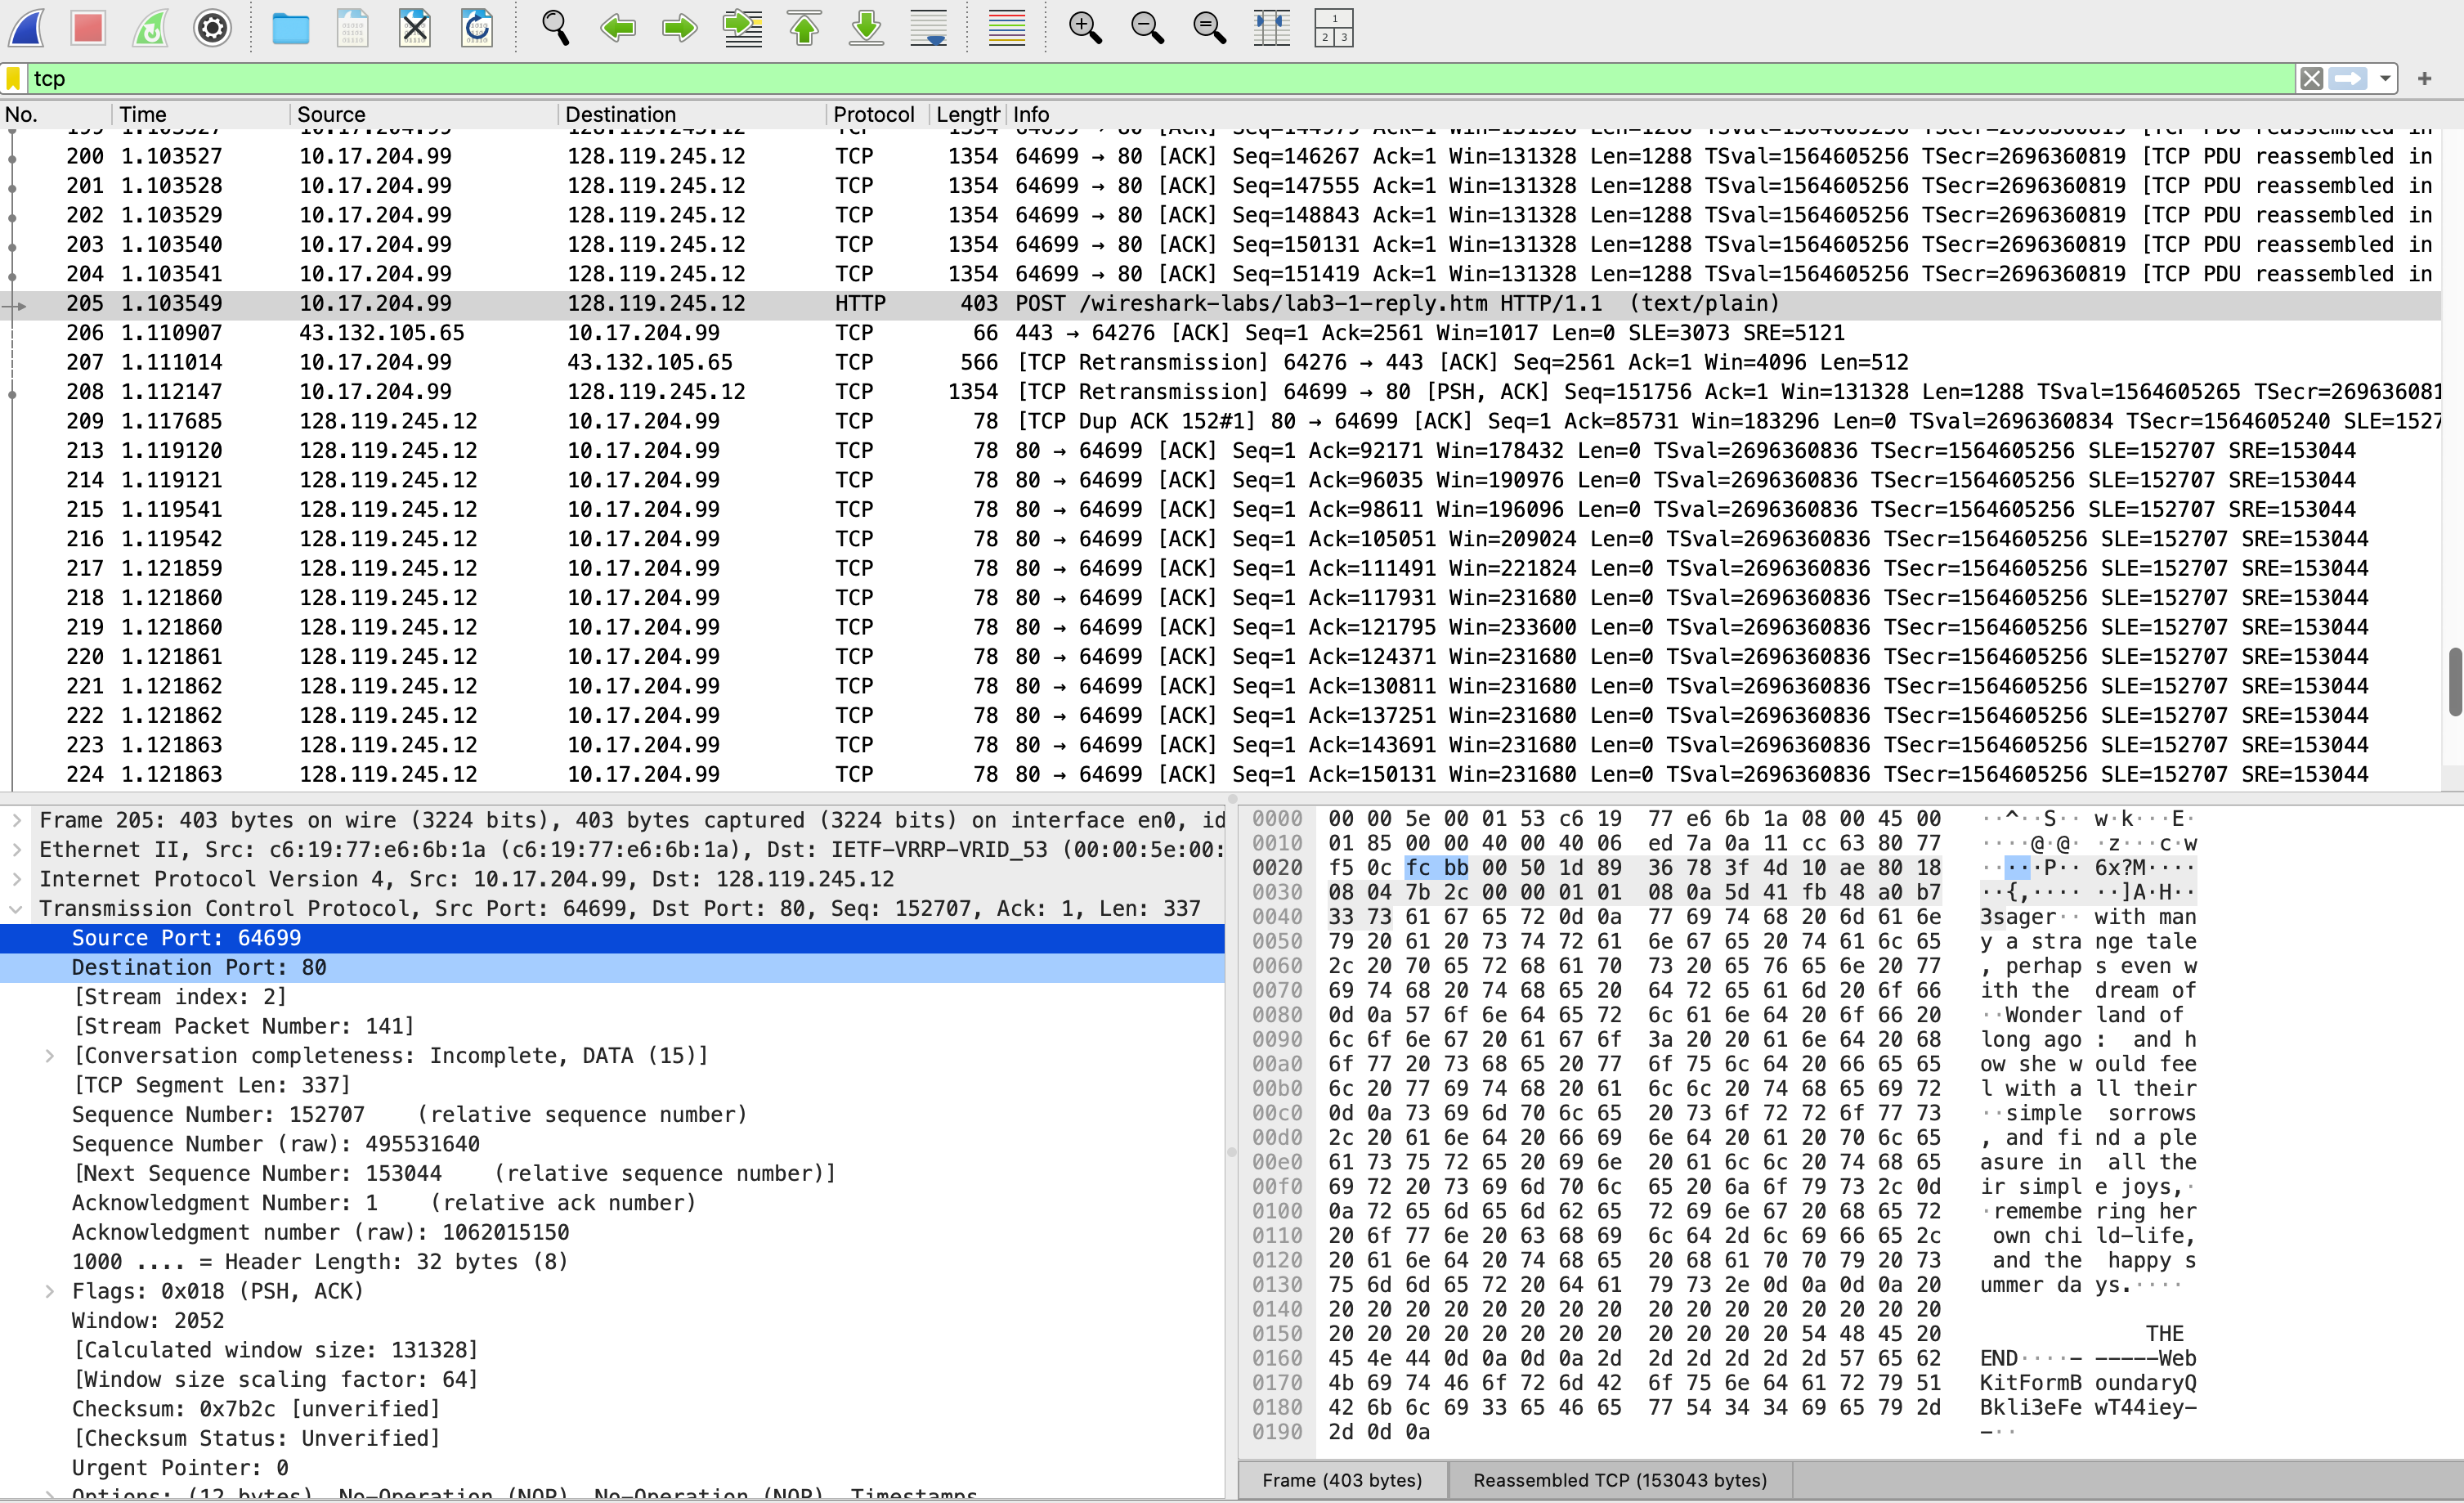
\includegraphics[width=0.8\textwidth]{2-1.png}
\end{figure}
\begin{figure}[H]
    \centering
    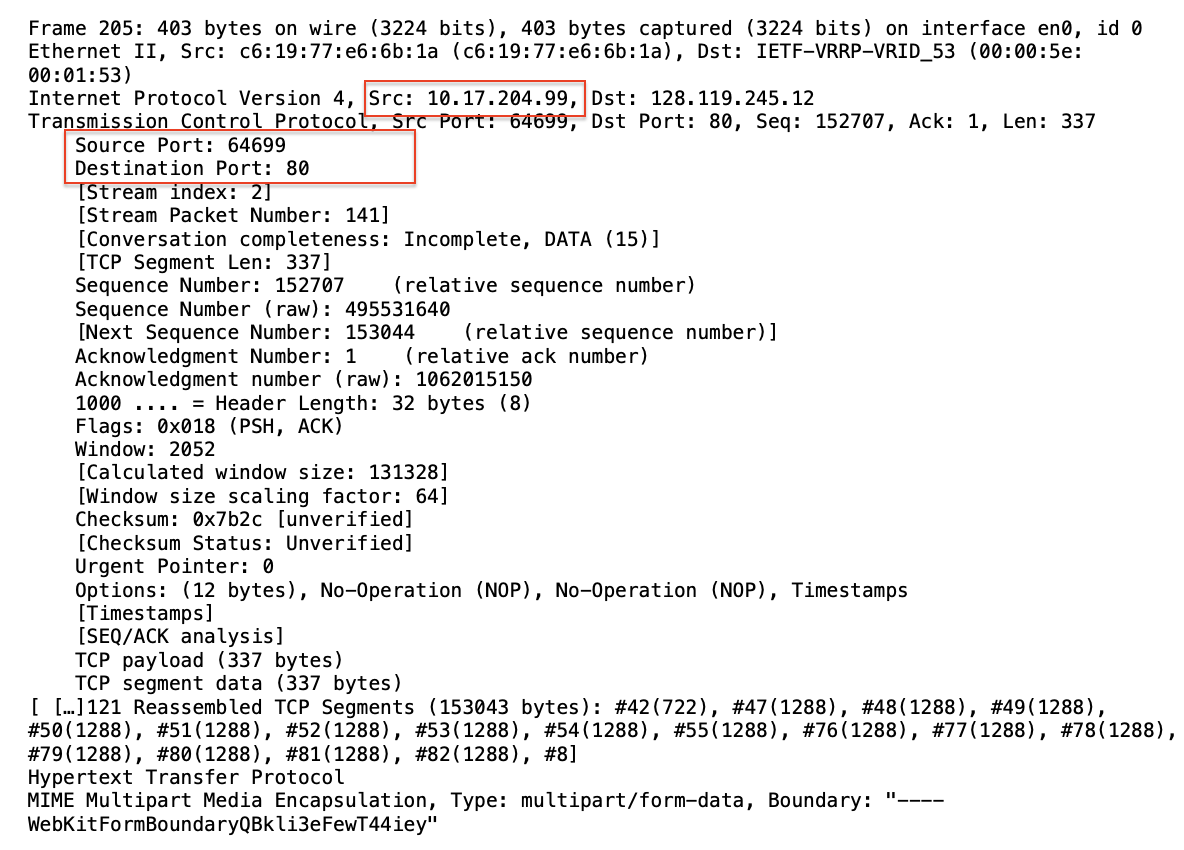
\includegraphics[width=0.8\textwidth]{2-2.png}
\end{figure}

\section{TCP Basics}
\subsection{}
\textbf{Answer}:The sequence number of the TCP SYN segment is 0.
The SYN flag is set to 1 in the segment, which identifies the segment as a SYN segment.
\begin{figure}[H]
    \centering
    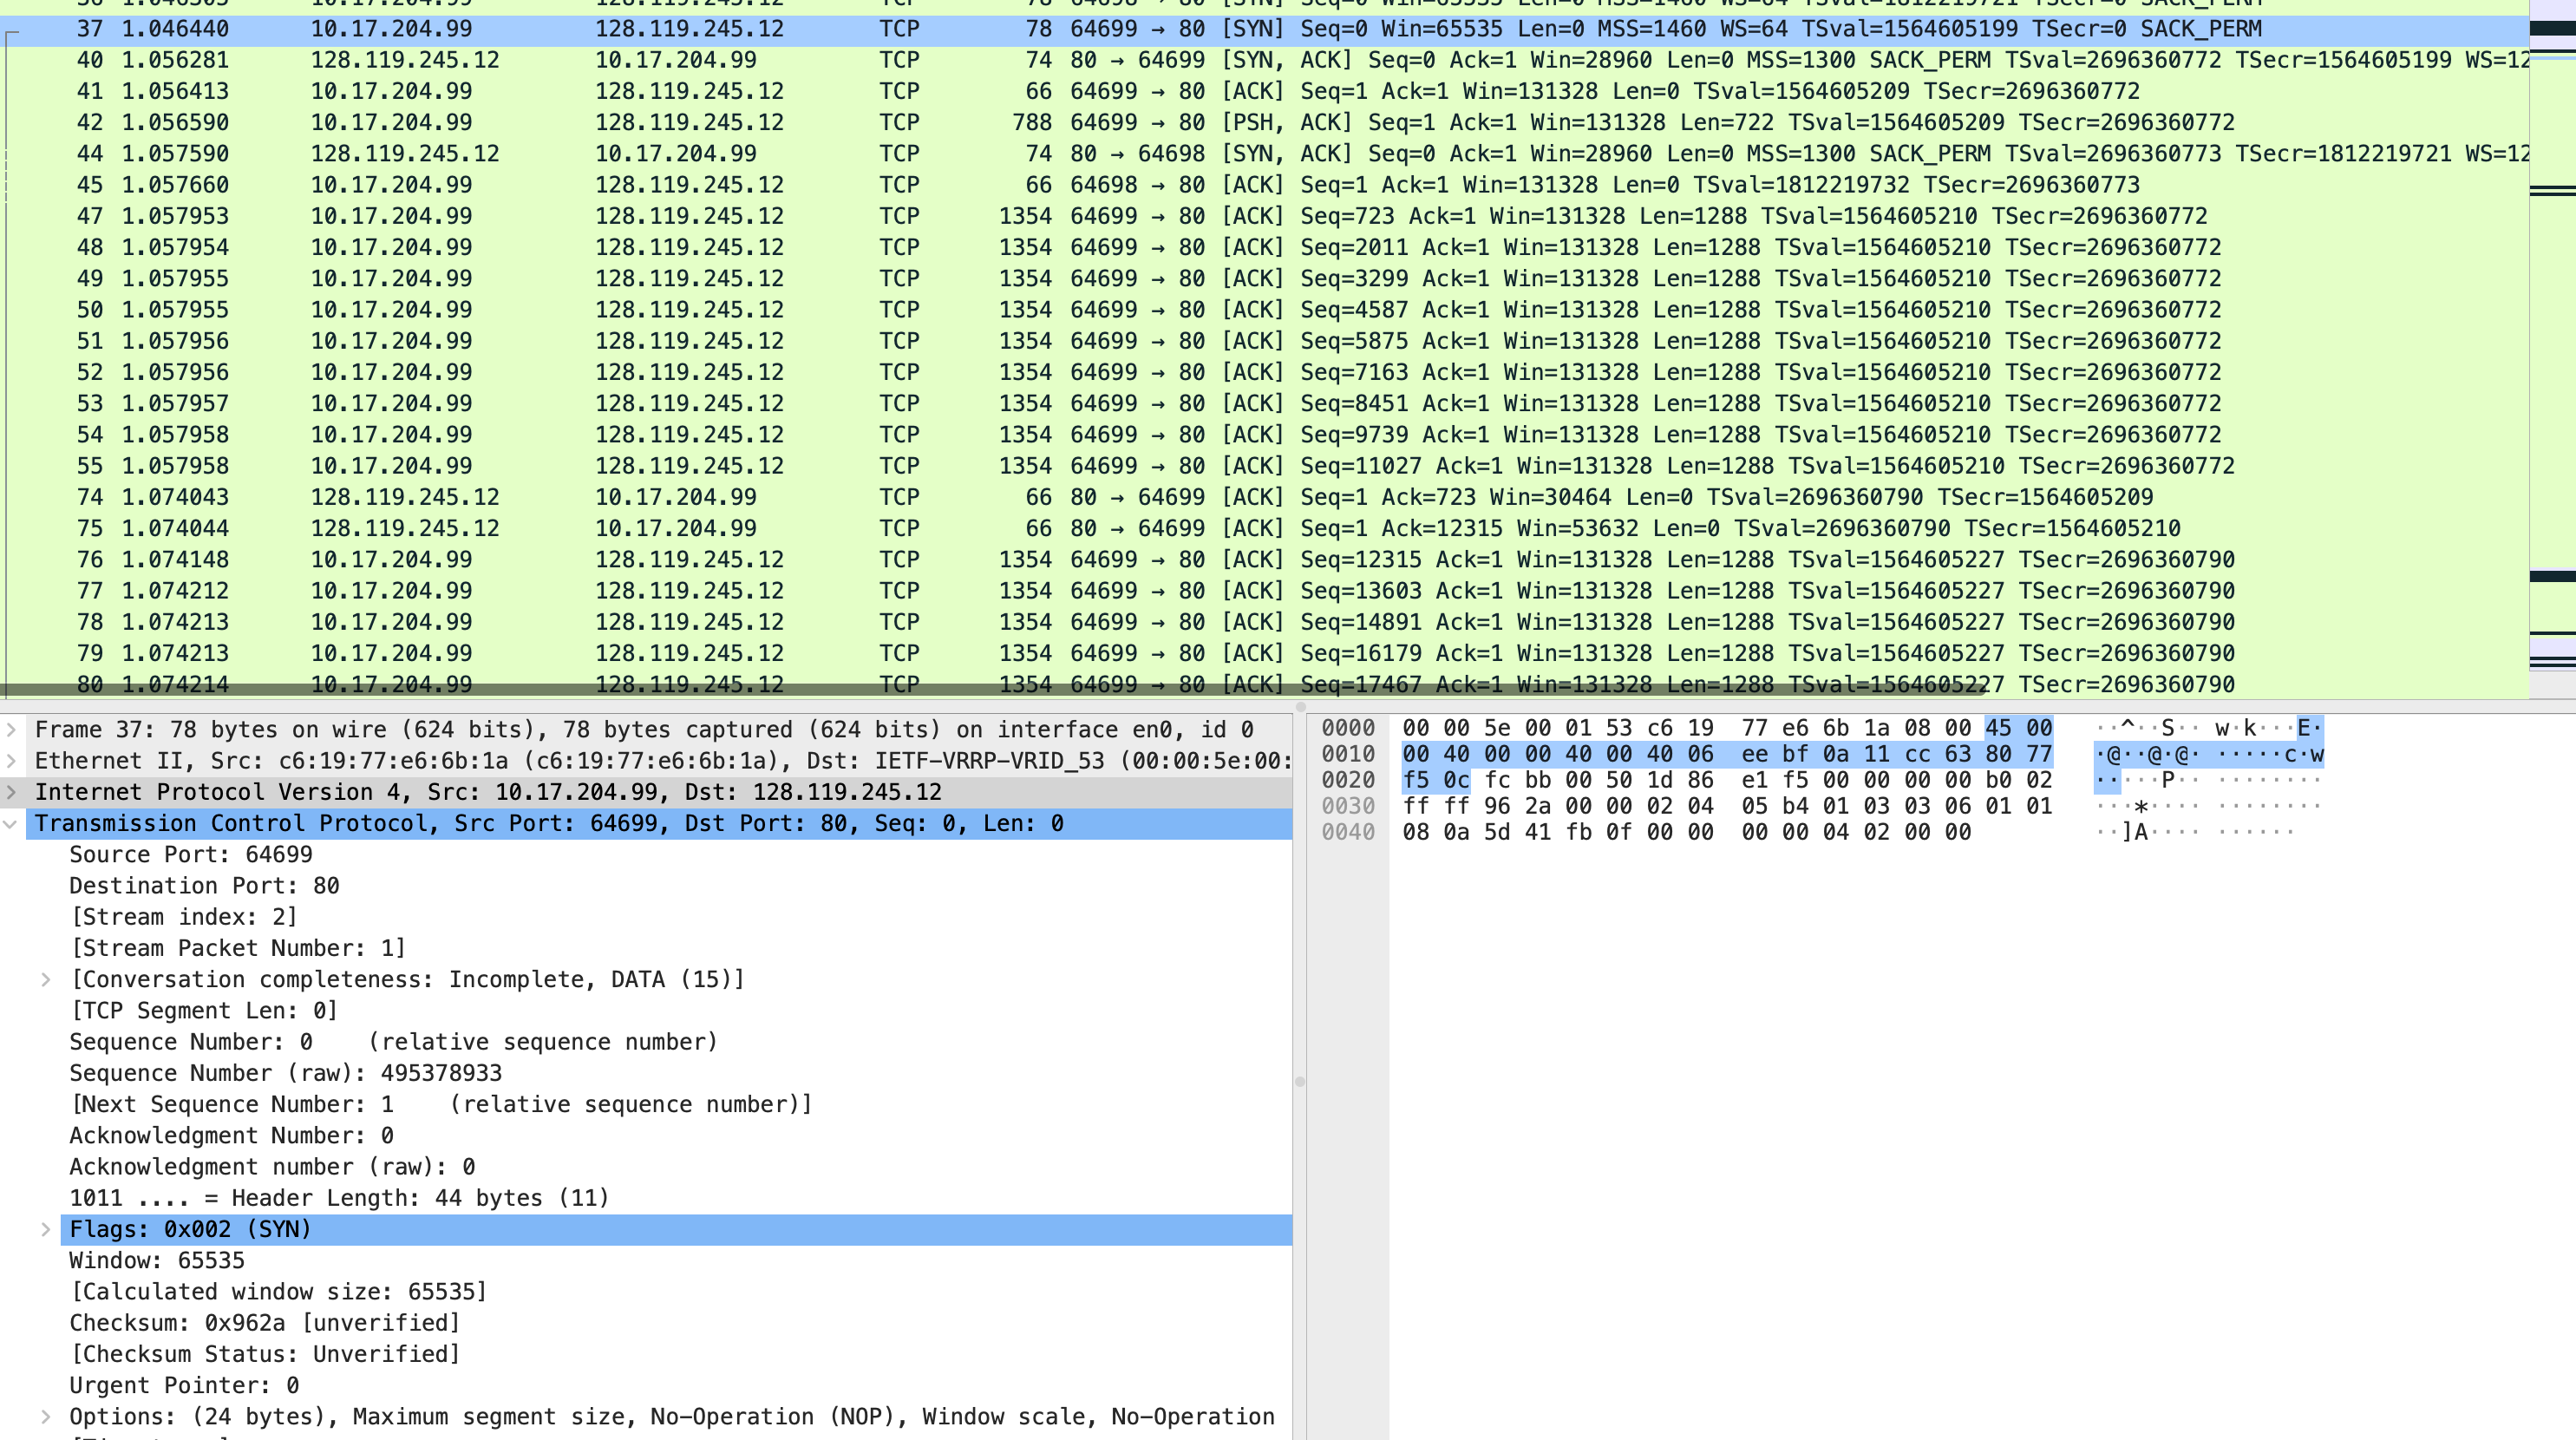
\includegraphics[width=0.8\textwidth]{4-1.png}
\end{figure}
\begin{figure}[H]
    \centering
    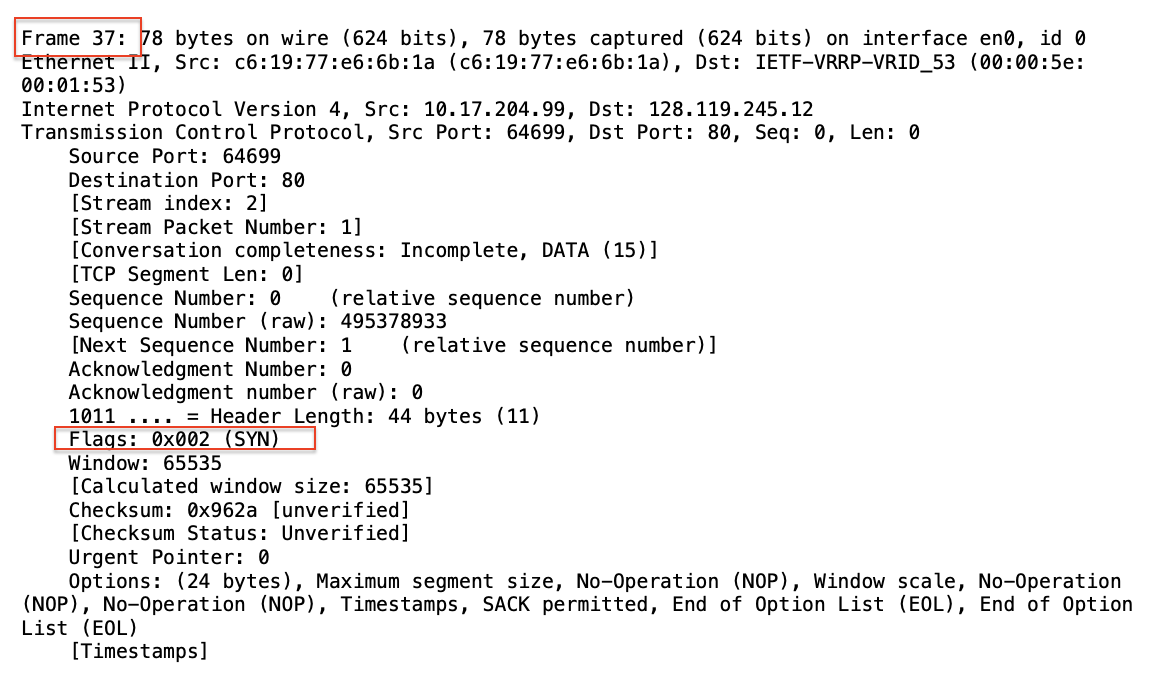
\includegraphics[width=0.8\textwidth]{4-2.png}
\end{figure}

\subsection{}
The sequence number of the SYNACK segment is 0.
The Acknowledgement field in the SYNACK segment is 1.
The Acknowledgement field in the SYNACK segment is determined by the sequence number of the SYN segment plus 1.
Both the SYN and ACK flags are set to 1 in the segment, which identifies the segment as a SYNACK segment.
\begin{figure}[H]
    \centering
    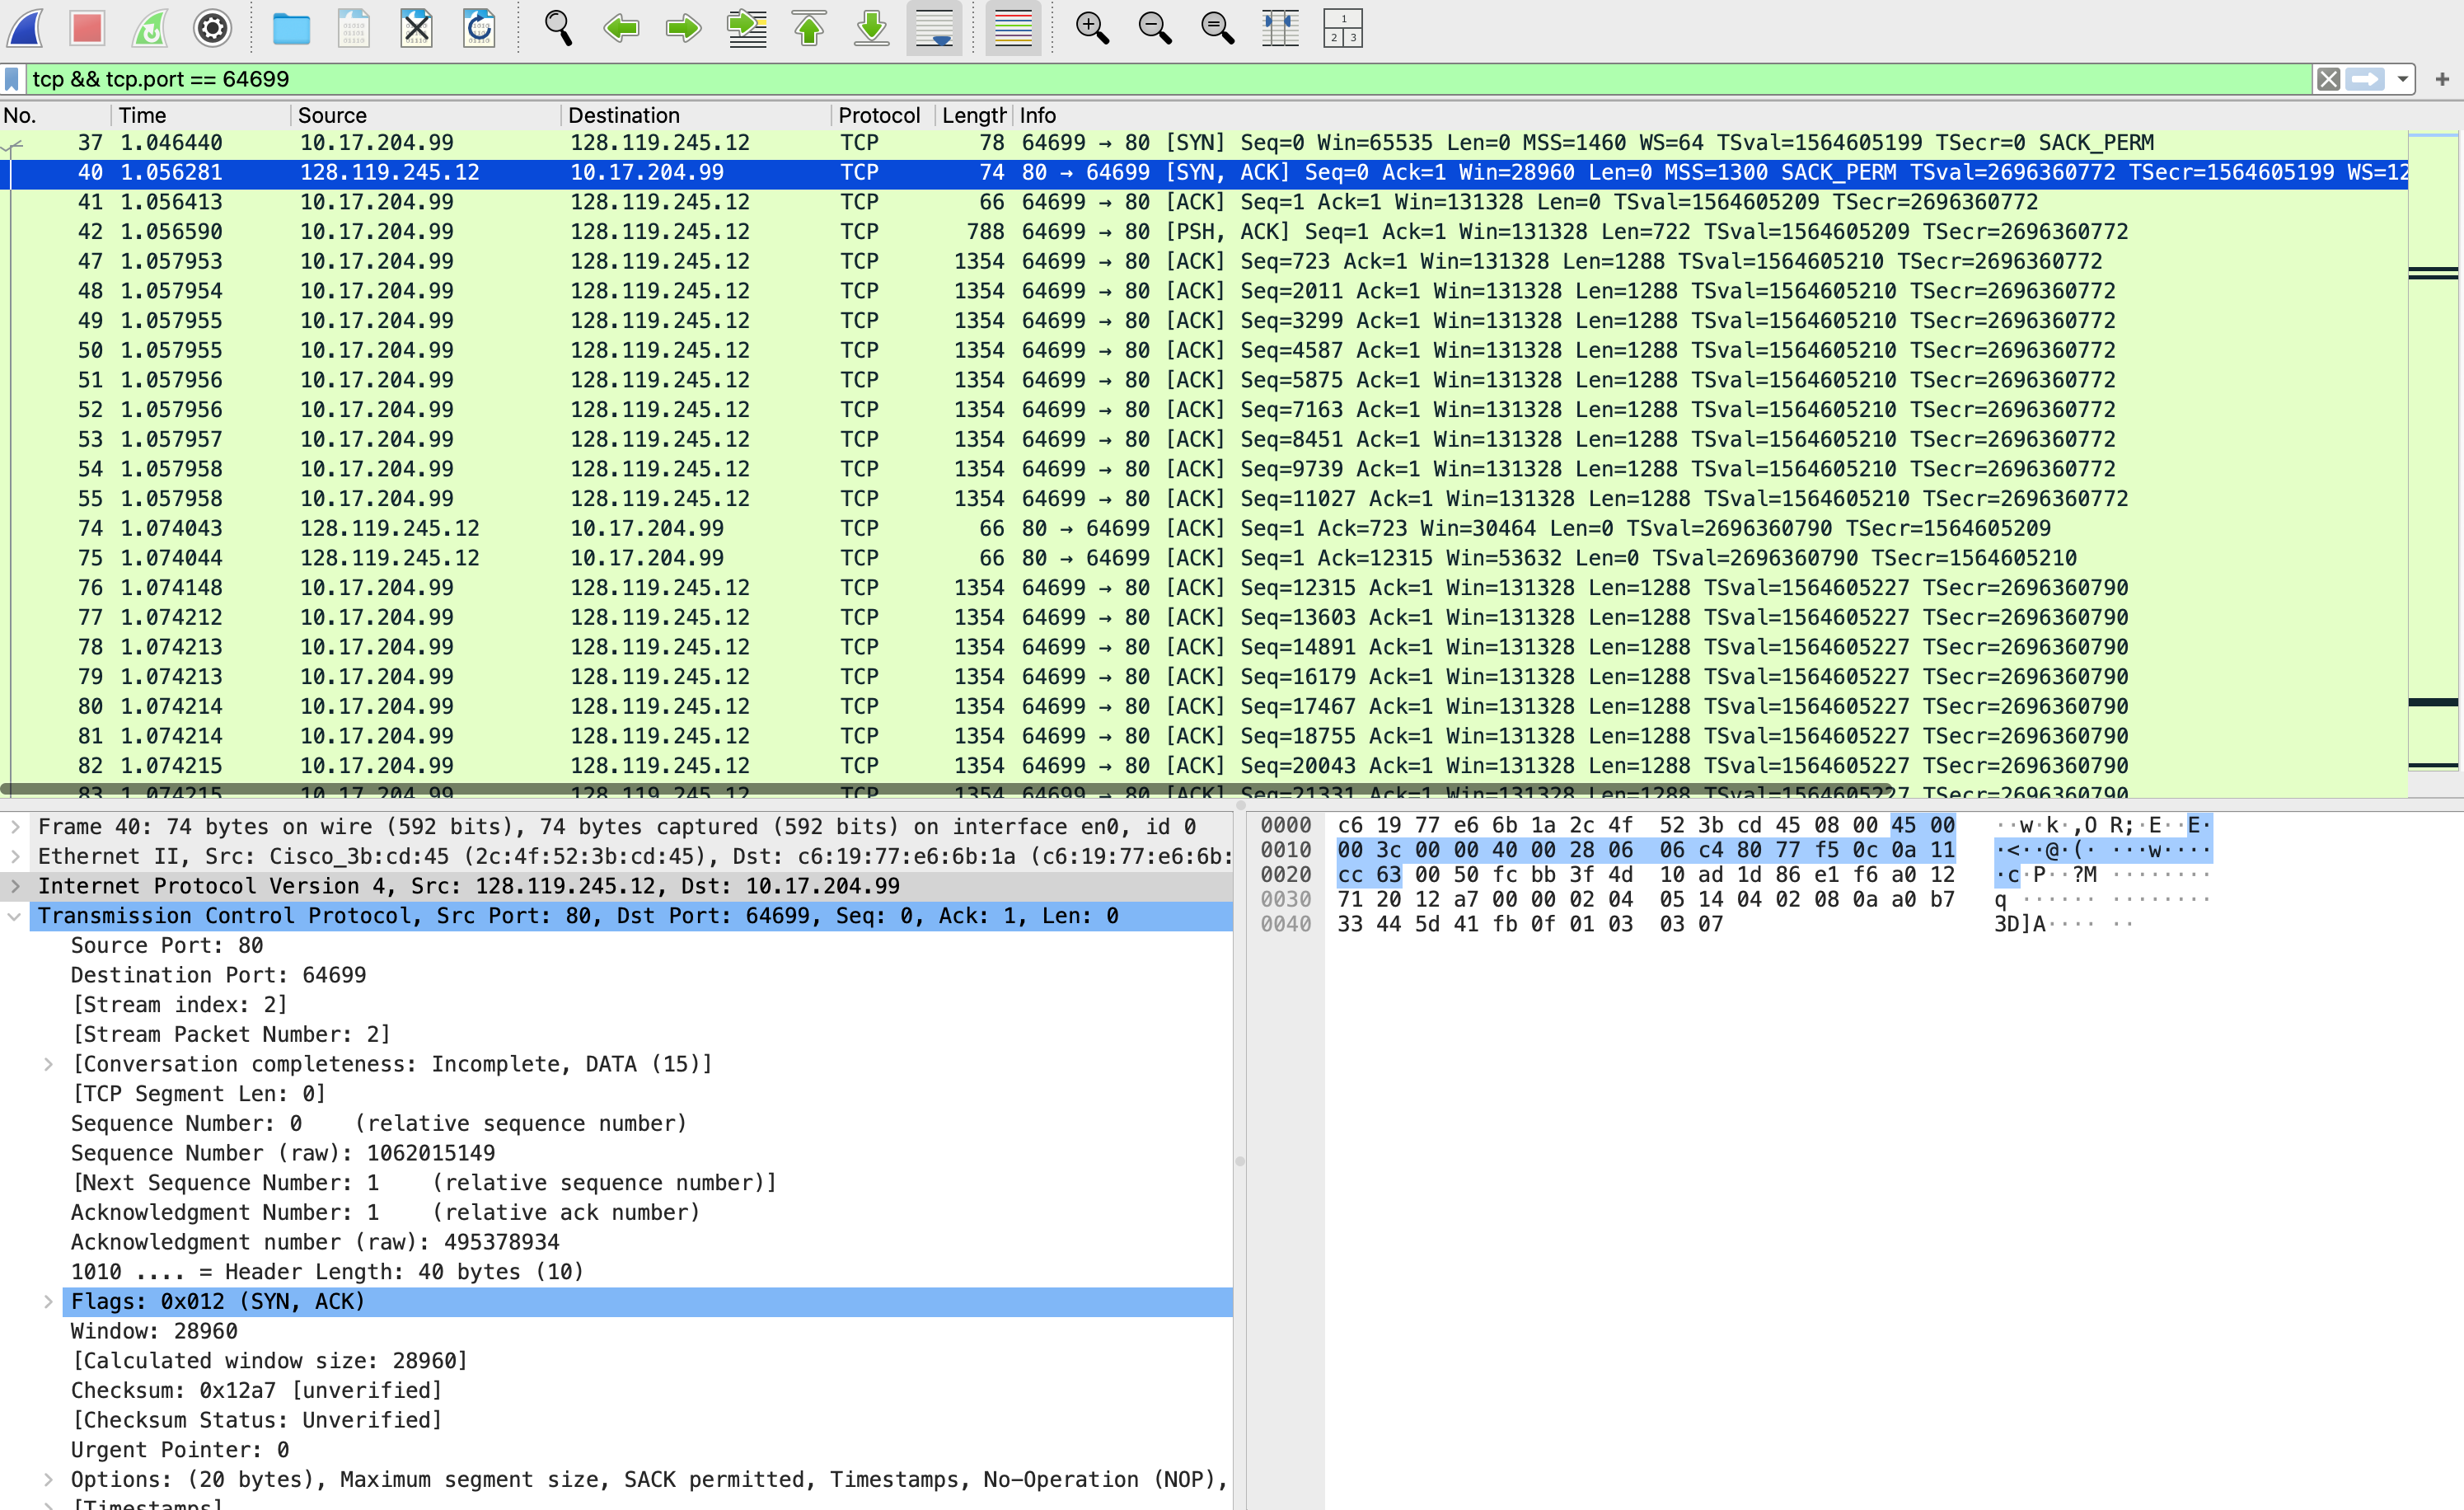
\includegraphics[width=0.8\textwidth]{5-1.png}
\end{figure}
\begin{figure}[H]
    \centering
    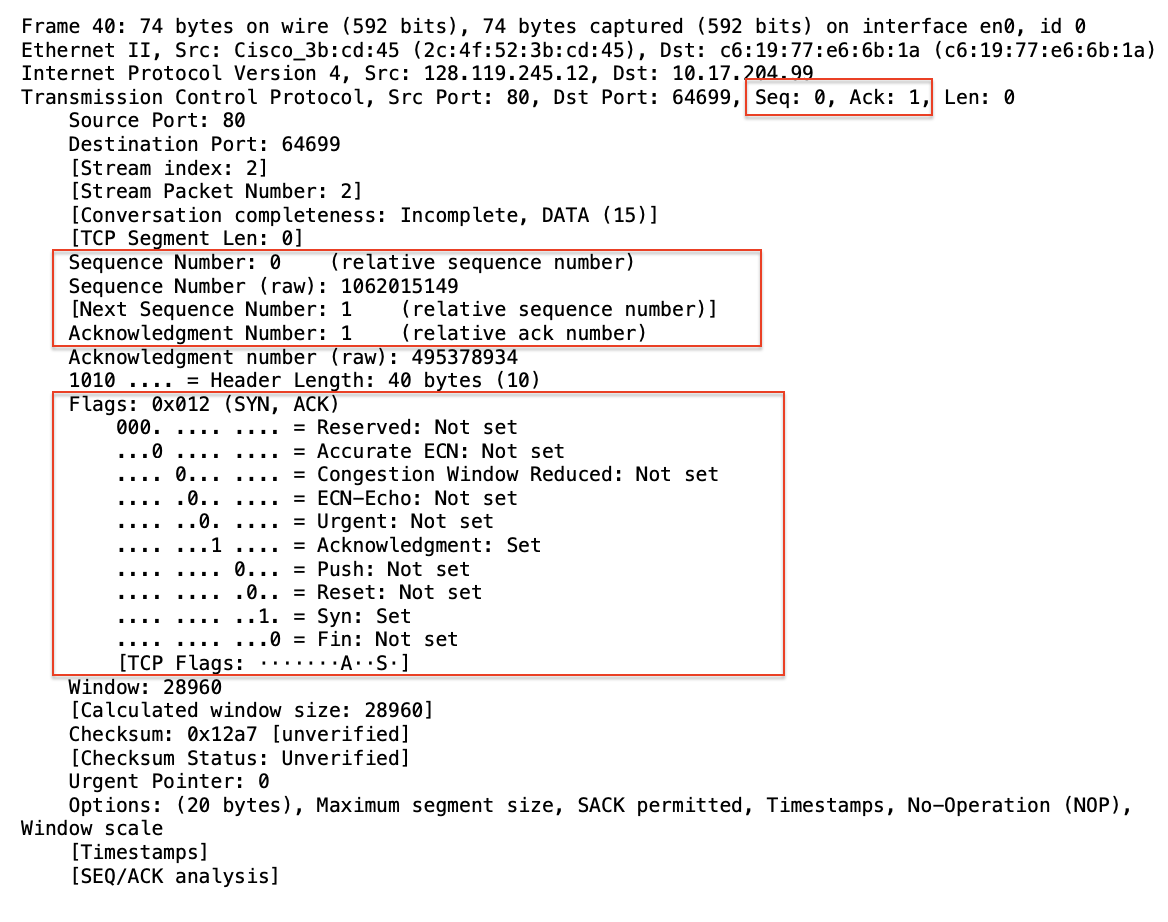
\includegraphics[width=0.8\textwidth]{5-2.png}
\end{figure}
\subsection{}
The sequence number of the TCP segment containing the HTTP POST command is 152707.
\begin{figure}[H]
    \centering
    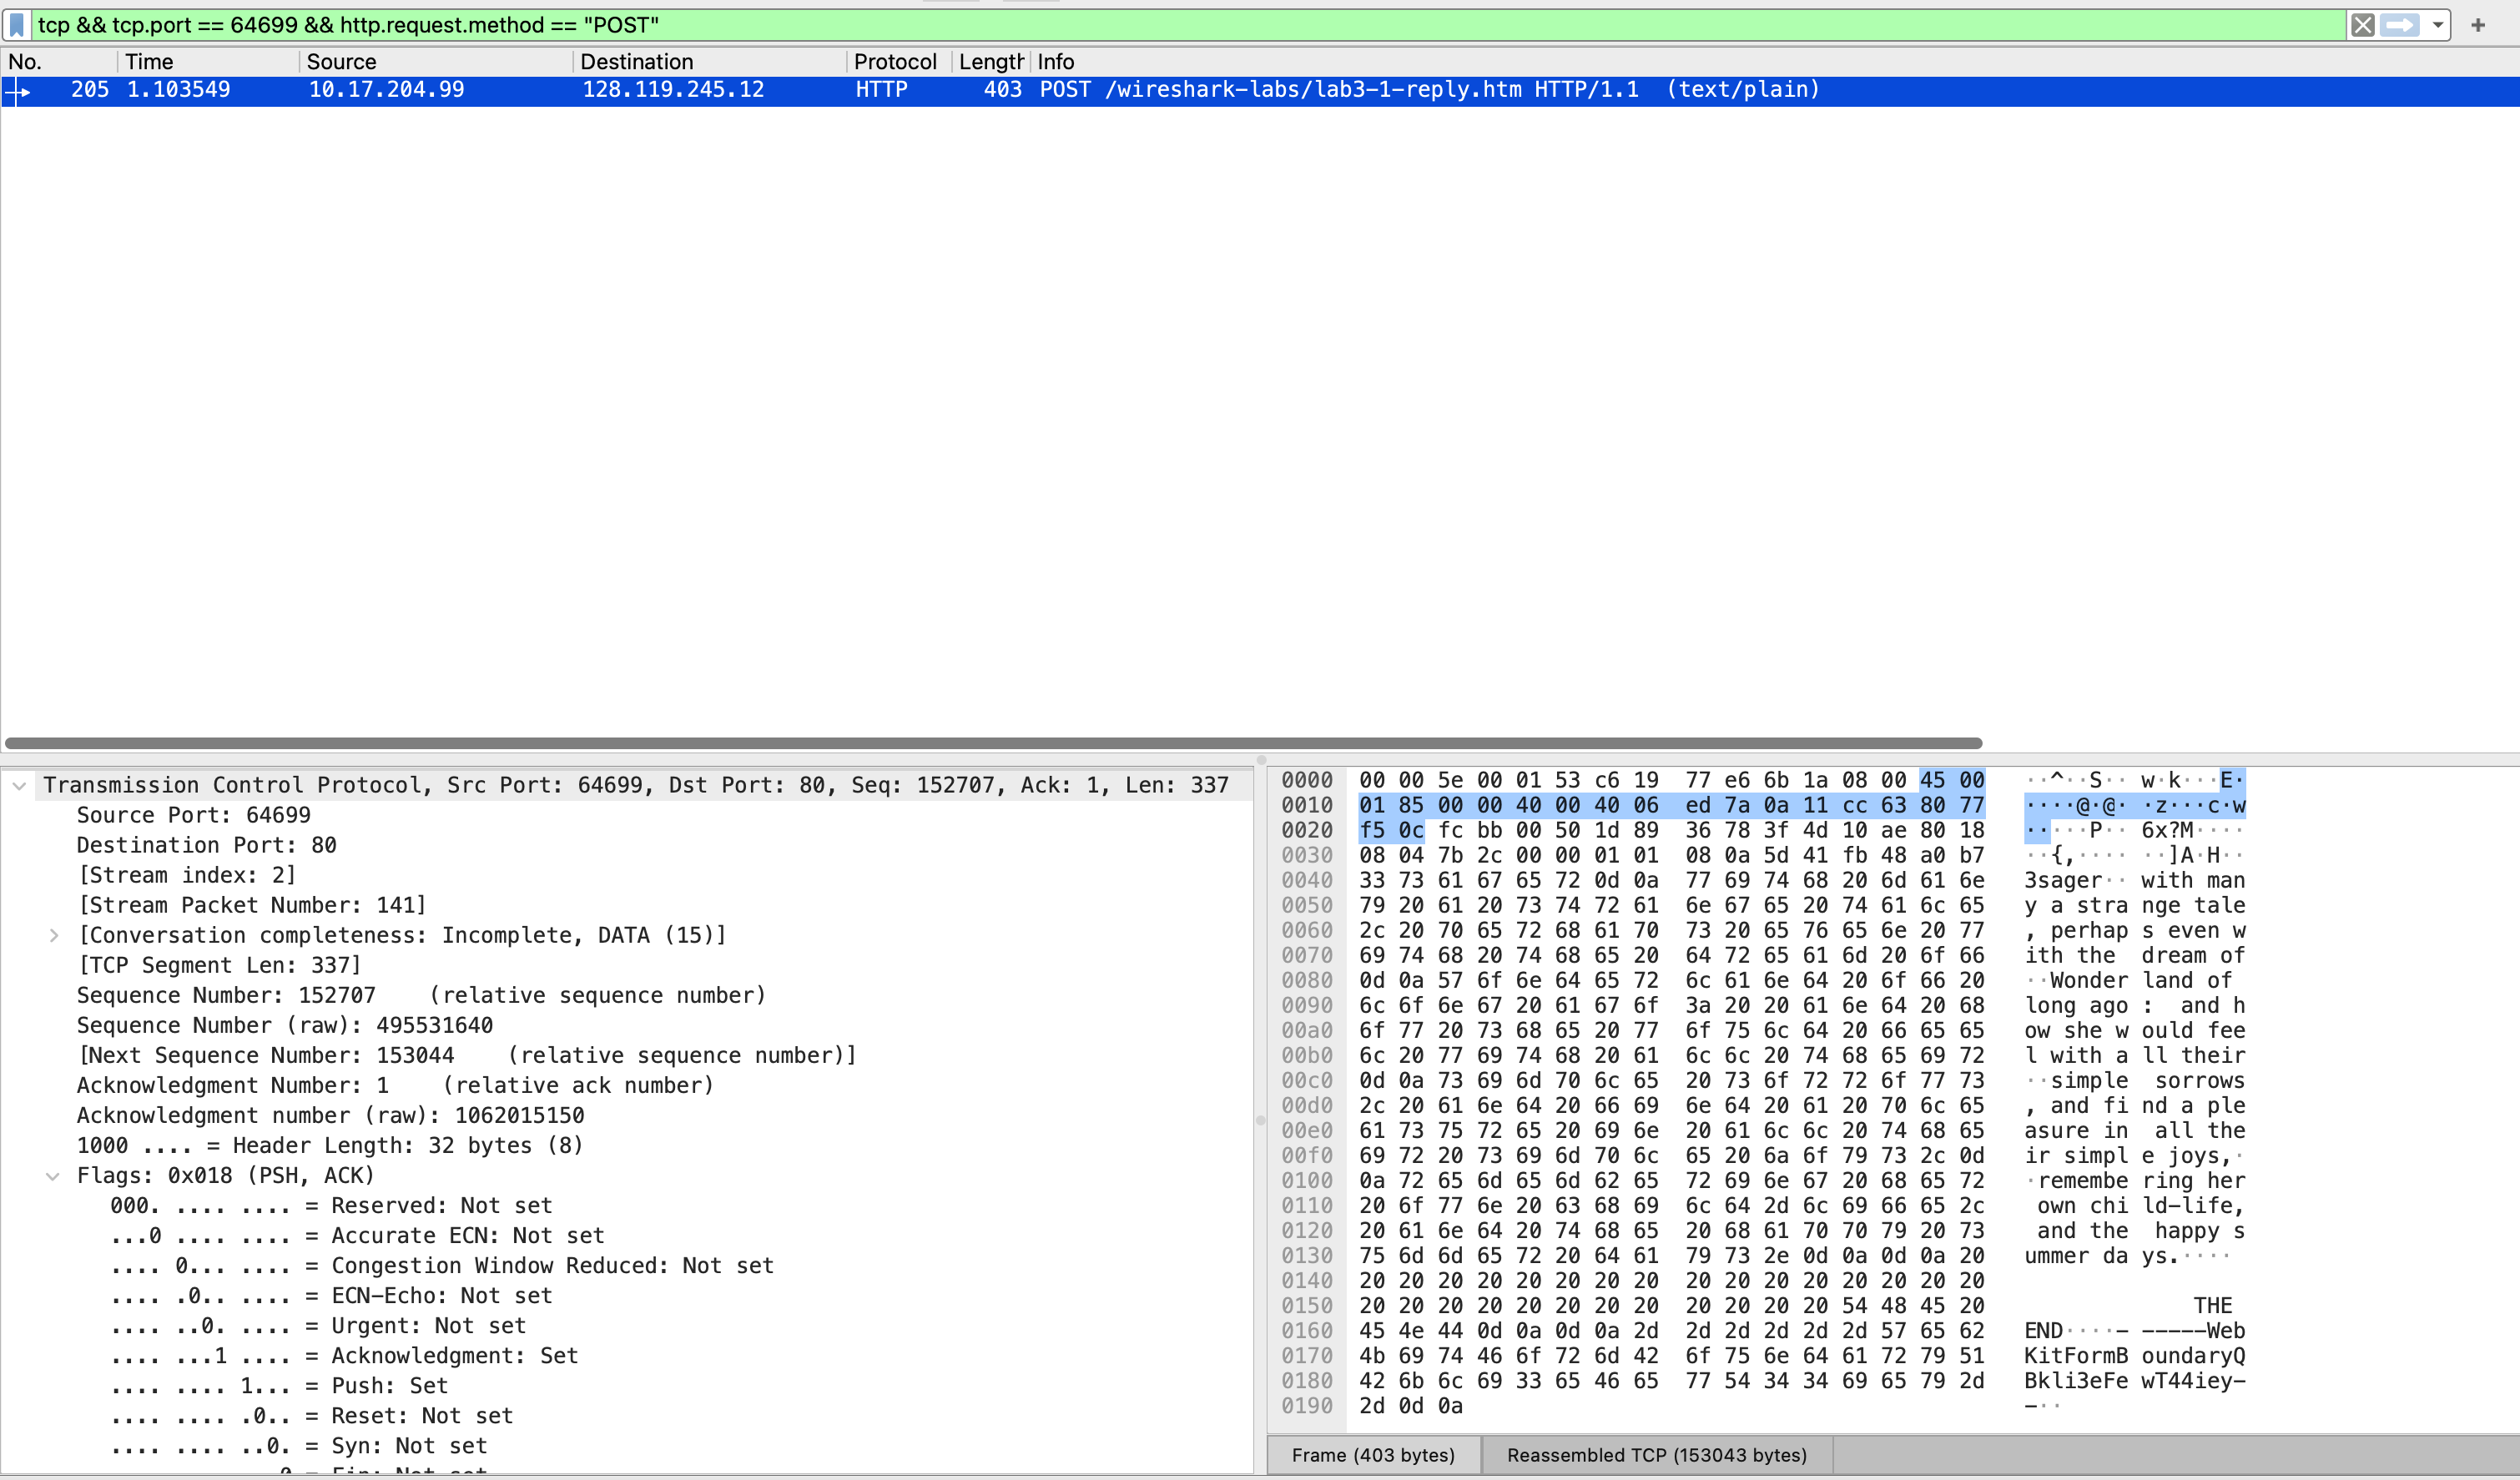
\includegraphics[width=0.8\textwidth]{6-1.png}
\end{figure}
\begin{figure}[H]
    \centering
    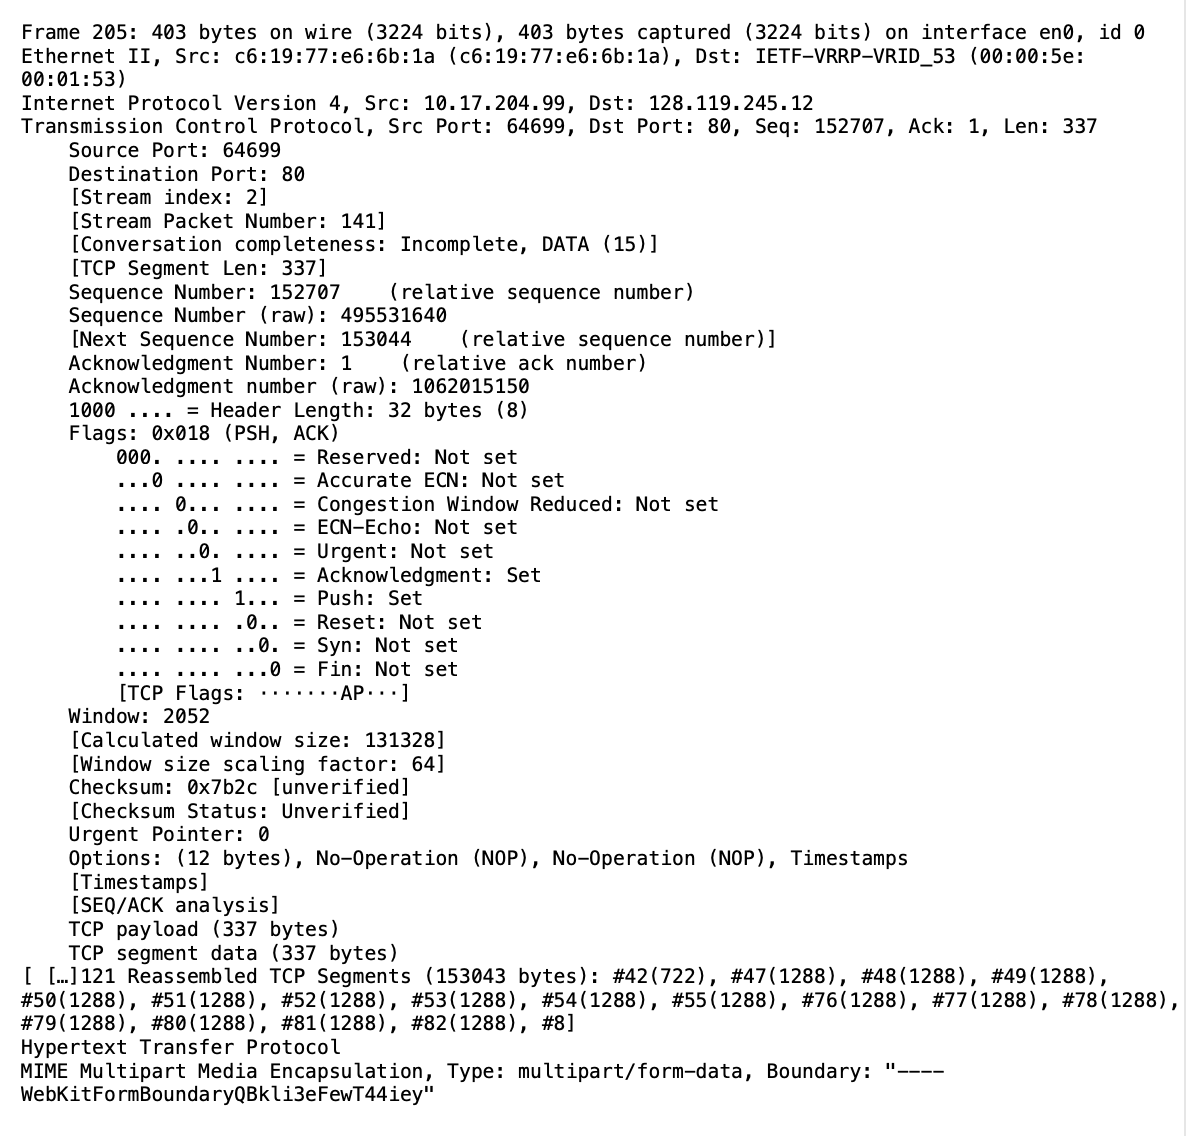
\includegraphics[width=0.8\textwidth]{6-2.png}
\end{figure}
\subsection{}
There is some problem in my own trace (retransmission) which affects the answer
for this question. So I use the tcpethereal-trace-1 to answer this question.
\begin{table}[h]
    \centering
    \begin{tabular}{clcccc}
        \toprule
        \textbf{Segment Number} & 
        \textbf{Seq} & 
        \textbf{Sent Time} & 
        \textbf{Who ACKs it?} & 
        \textbf{ACK Received Time} & 
        \textbf{RTT (s)} \\
        \midrule
        1 (Frame 199) & 164041 & 5.297341 & Frame202 (Ack=164091)& 5.455830 & \textbf{0.158489} \\
        2 (Frame 200)& 1 & 5.389471 & 	Frame206 (Ack=731)& 5.651141 & \textbf{0.26167} \\
        3 (Frame 201) & 1 & 5.447887 & 	Frame206 (Ack=731)& 5.651141 & \textbf{0.203254} \\
        4 (Frame 202) & 1 & 5.455830 & Frame206 (Ack=731)& 5.651141	 & \textbf{0.195311} \\
        5 (Frame 203) & 1 & 5.461175 & Frame206 (Ack=731)& 5.651141	 & \textbf{0.189966} \\
        6 (Frame 206) & 164091 & 5.651141 & Not detected & \textbf{N/A} & \textbf{N/A} \\
        \bottomrule
    \end{tabular}
    \caption{Sequence Numbers, Timestamps, and RTT Values of First Six TCP Segments}
    \label{tab:rtt_values}
\end{table}

\begin{figure}[H]
    \centering
    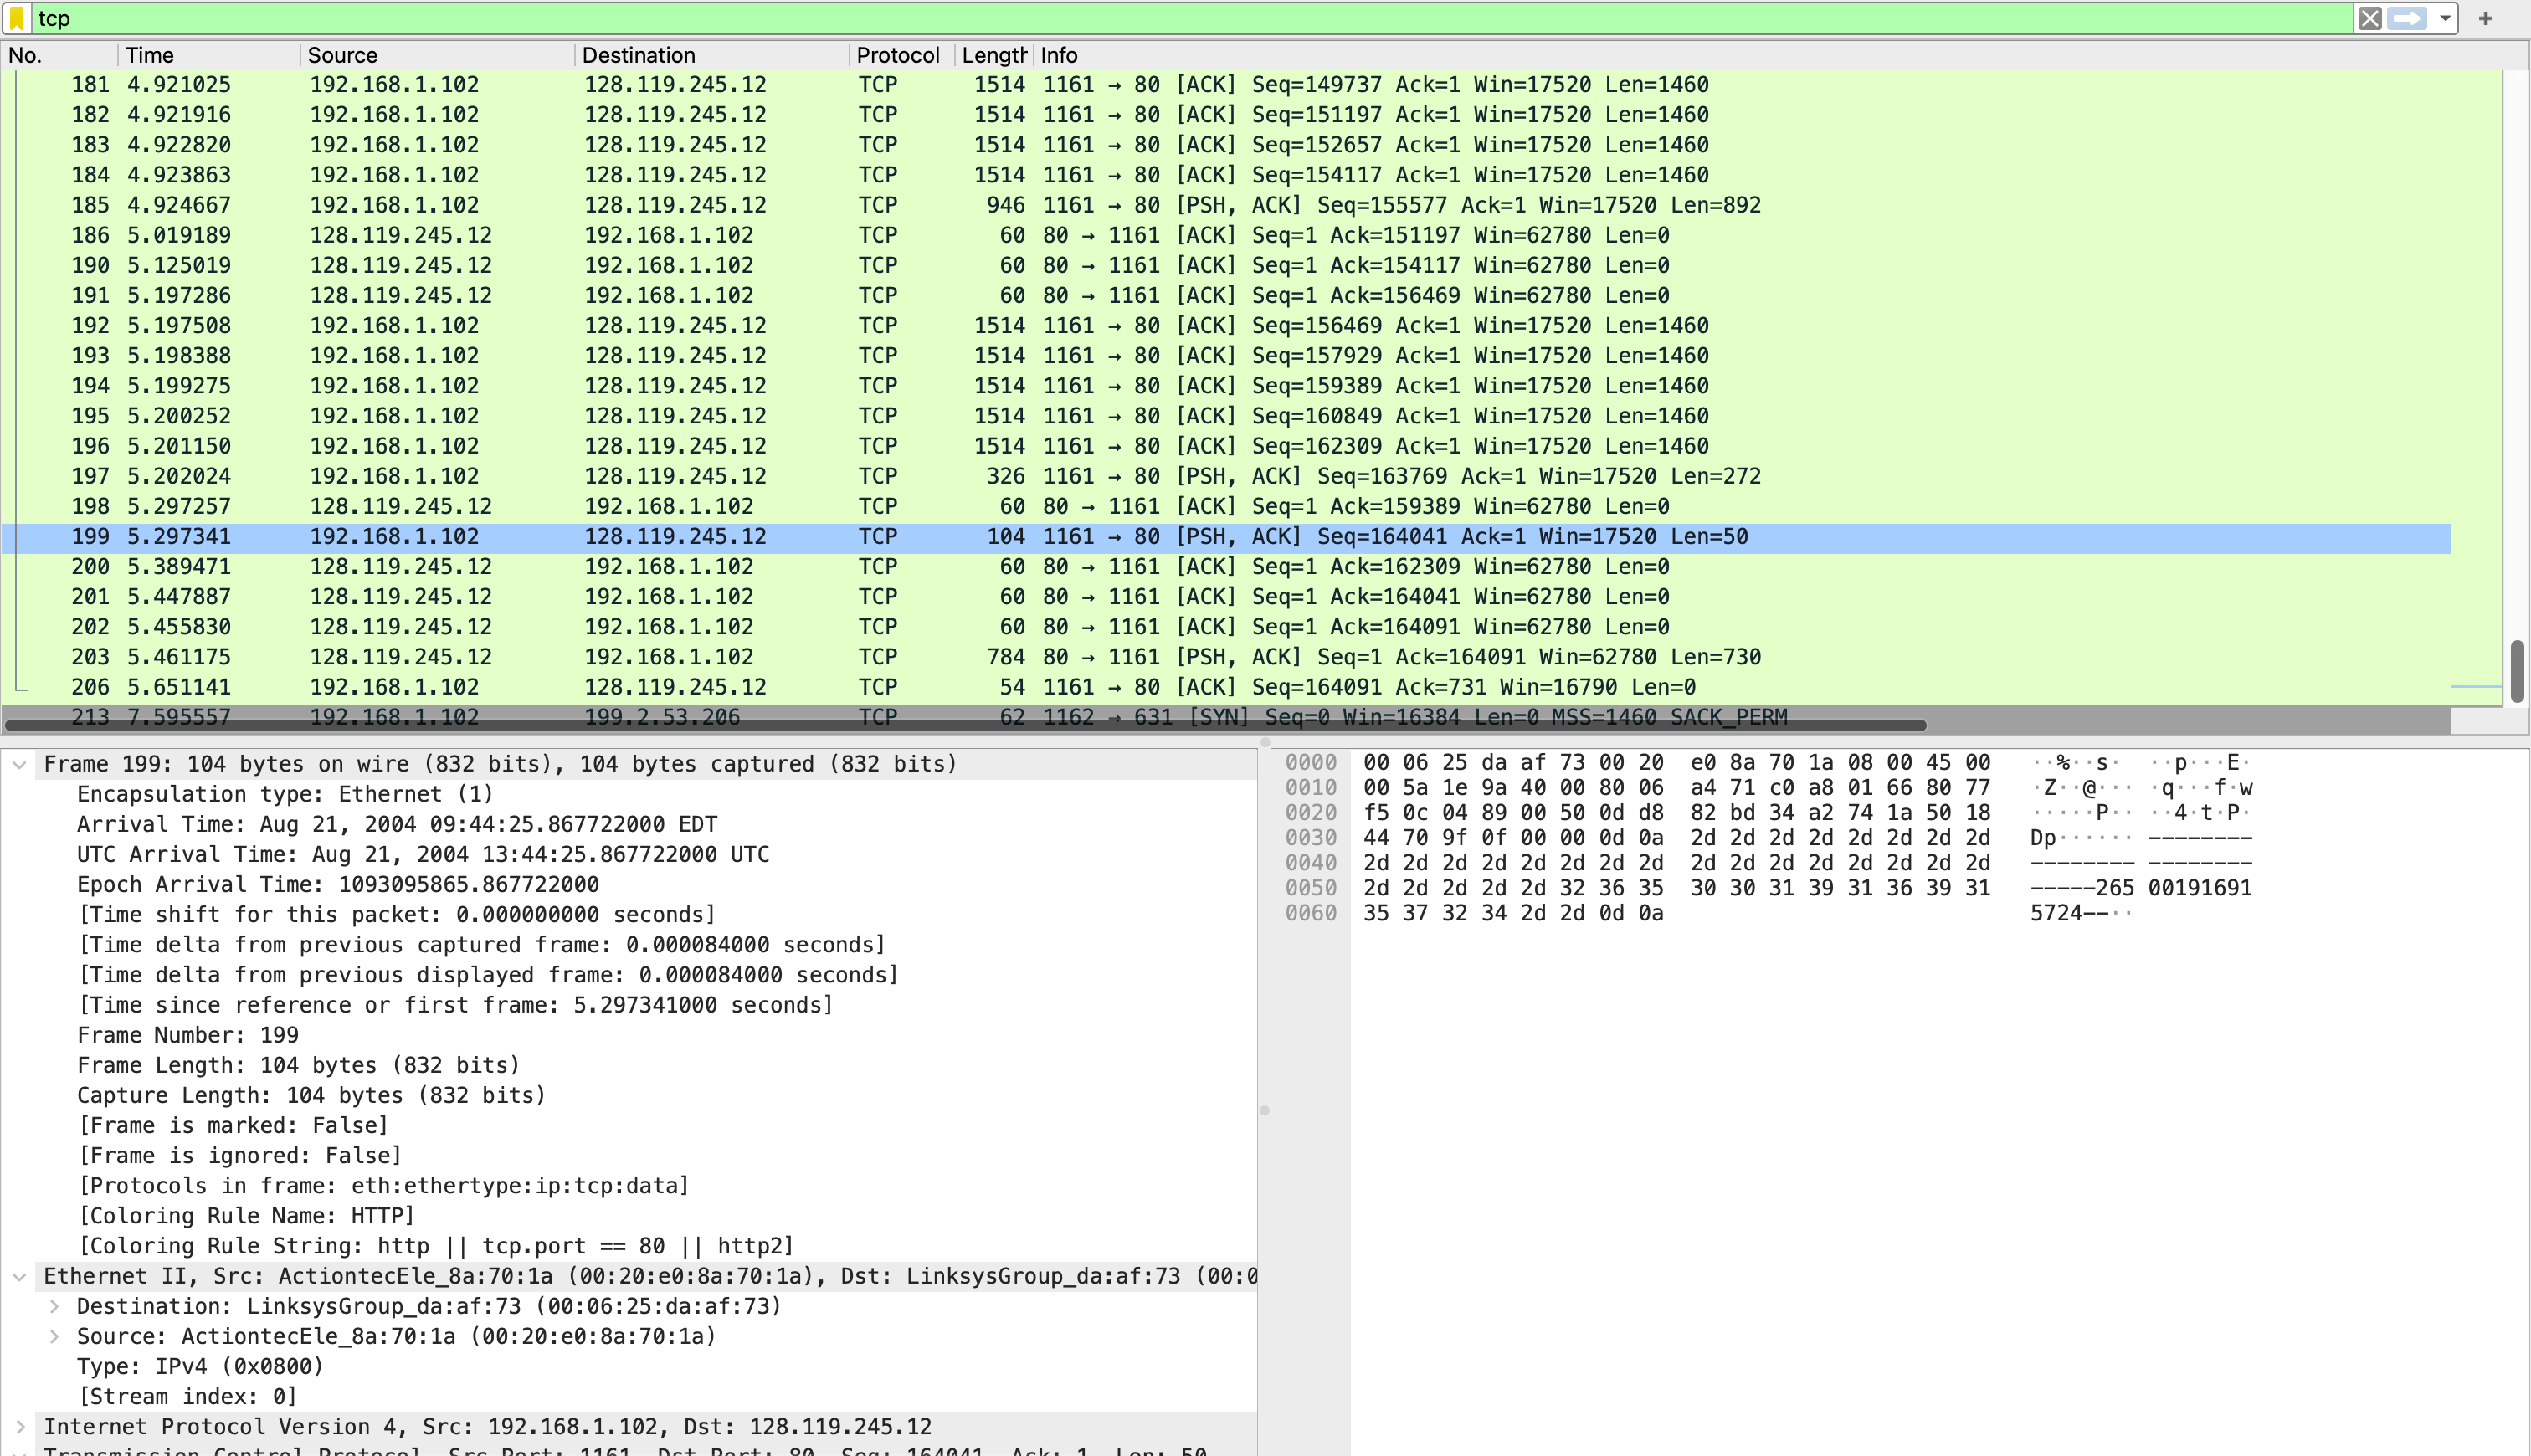
\includegraphics[width=1\textwidth]{7-1.png}
\end{figure}
Since in the example trace, I cannot find the ACK segment for the last segment (the next segment frame 213
is on the different TCP because the port number is different), so I cannot calculate the RTT for the last segment.
\\\textbf{Calculating the Estimated RTT}:
\begin{align*}
    \text{EstimatedRTT} &= (1-\alpha) \times \text{EstimatedRTT} + \alpha \times \text{SampleRTT} \\
\end{align*}
where $\alpha = 0.125$, so $1-\alpha = 0.875$.
\begin{align*}
    \text{EstimatedRTT 199} &= 0.158489 \\
    \text{EstimatedRTT 200} &= 0.875 \times 0.158489 + 0.125 \times 0.26167 = 0.1714 \\
    \text{EstimatedRTT 201} &= 0.875 \times 0.1714 + 0.125 \times 0.203254 = 0.1754 \\
    \text{EstimatedRTT 202} &= 0.875 \times 0.1754 + 0.125 \times 0.195311 = 0.1779 \\
    \text{EstimatedRTT 203} &= 0.875 \times 0.1779 + 0.125 \times 0.189966 = 0.1794 \\
    \text{EstimatedRTT 203} &= \text{N/A} \\
\end{align*}
\subsection{}
the length of each of the first six TCP segments:
\begin{table}[H]
    \centering
    \begin{tabular}{cccc}
        \toprule
        \textbf{Segment Number} & 
        \textbf{Length} & 
        \textbf{Segment Number} & 
        \textbf{Length} \\
        \midrule
        1 (Frame 199) & 50 & 4 (Frame 202) & 0 \\
        2 (Frame 200) & 0 & 5 (Frame 203) & 730 \\
        3 (Frame 201) & 0 & 6 (Frame 206) & 0 \\
        \bottomrule
    \end{tabular}
    \caption{Length of First Six TCP Segments}
    \label{tab:length_values}
\end{table}

\subsection{}
I will turn back to my own trace to answer this question 
(9.What is the minimum amount of available buffer space advertised at the received for the entire trace? Does the lack of receiver buffer space ever throttle the sender?)
and the following questions.
\\The minimum amount of available buffer space advertised at the receiver for the entire trace is 238
bytes. And the calculated window size is 30464 bytes. According to the next
line, we can find that the lack of receiver buffer space does not throttle the sender because the
window size is larger and the sender does not have to wait for the receiver to free up buffer space.
\begin{figure}[H]
    \centering
    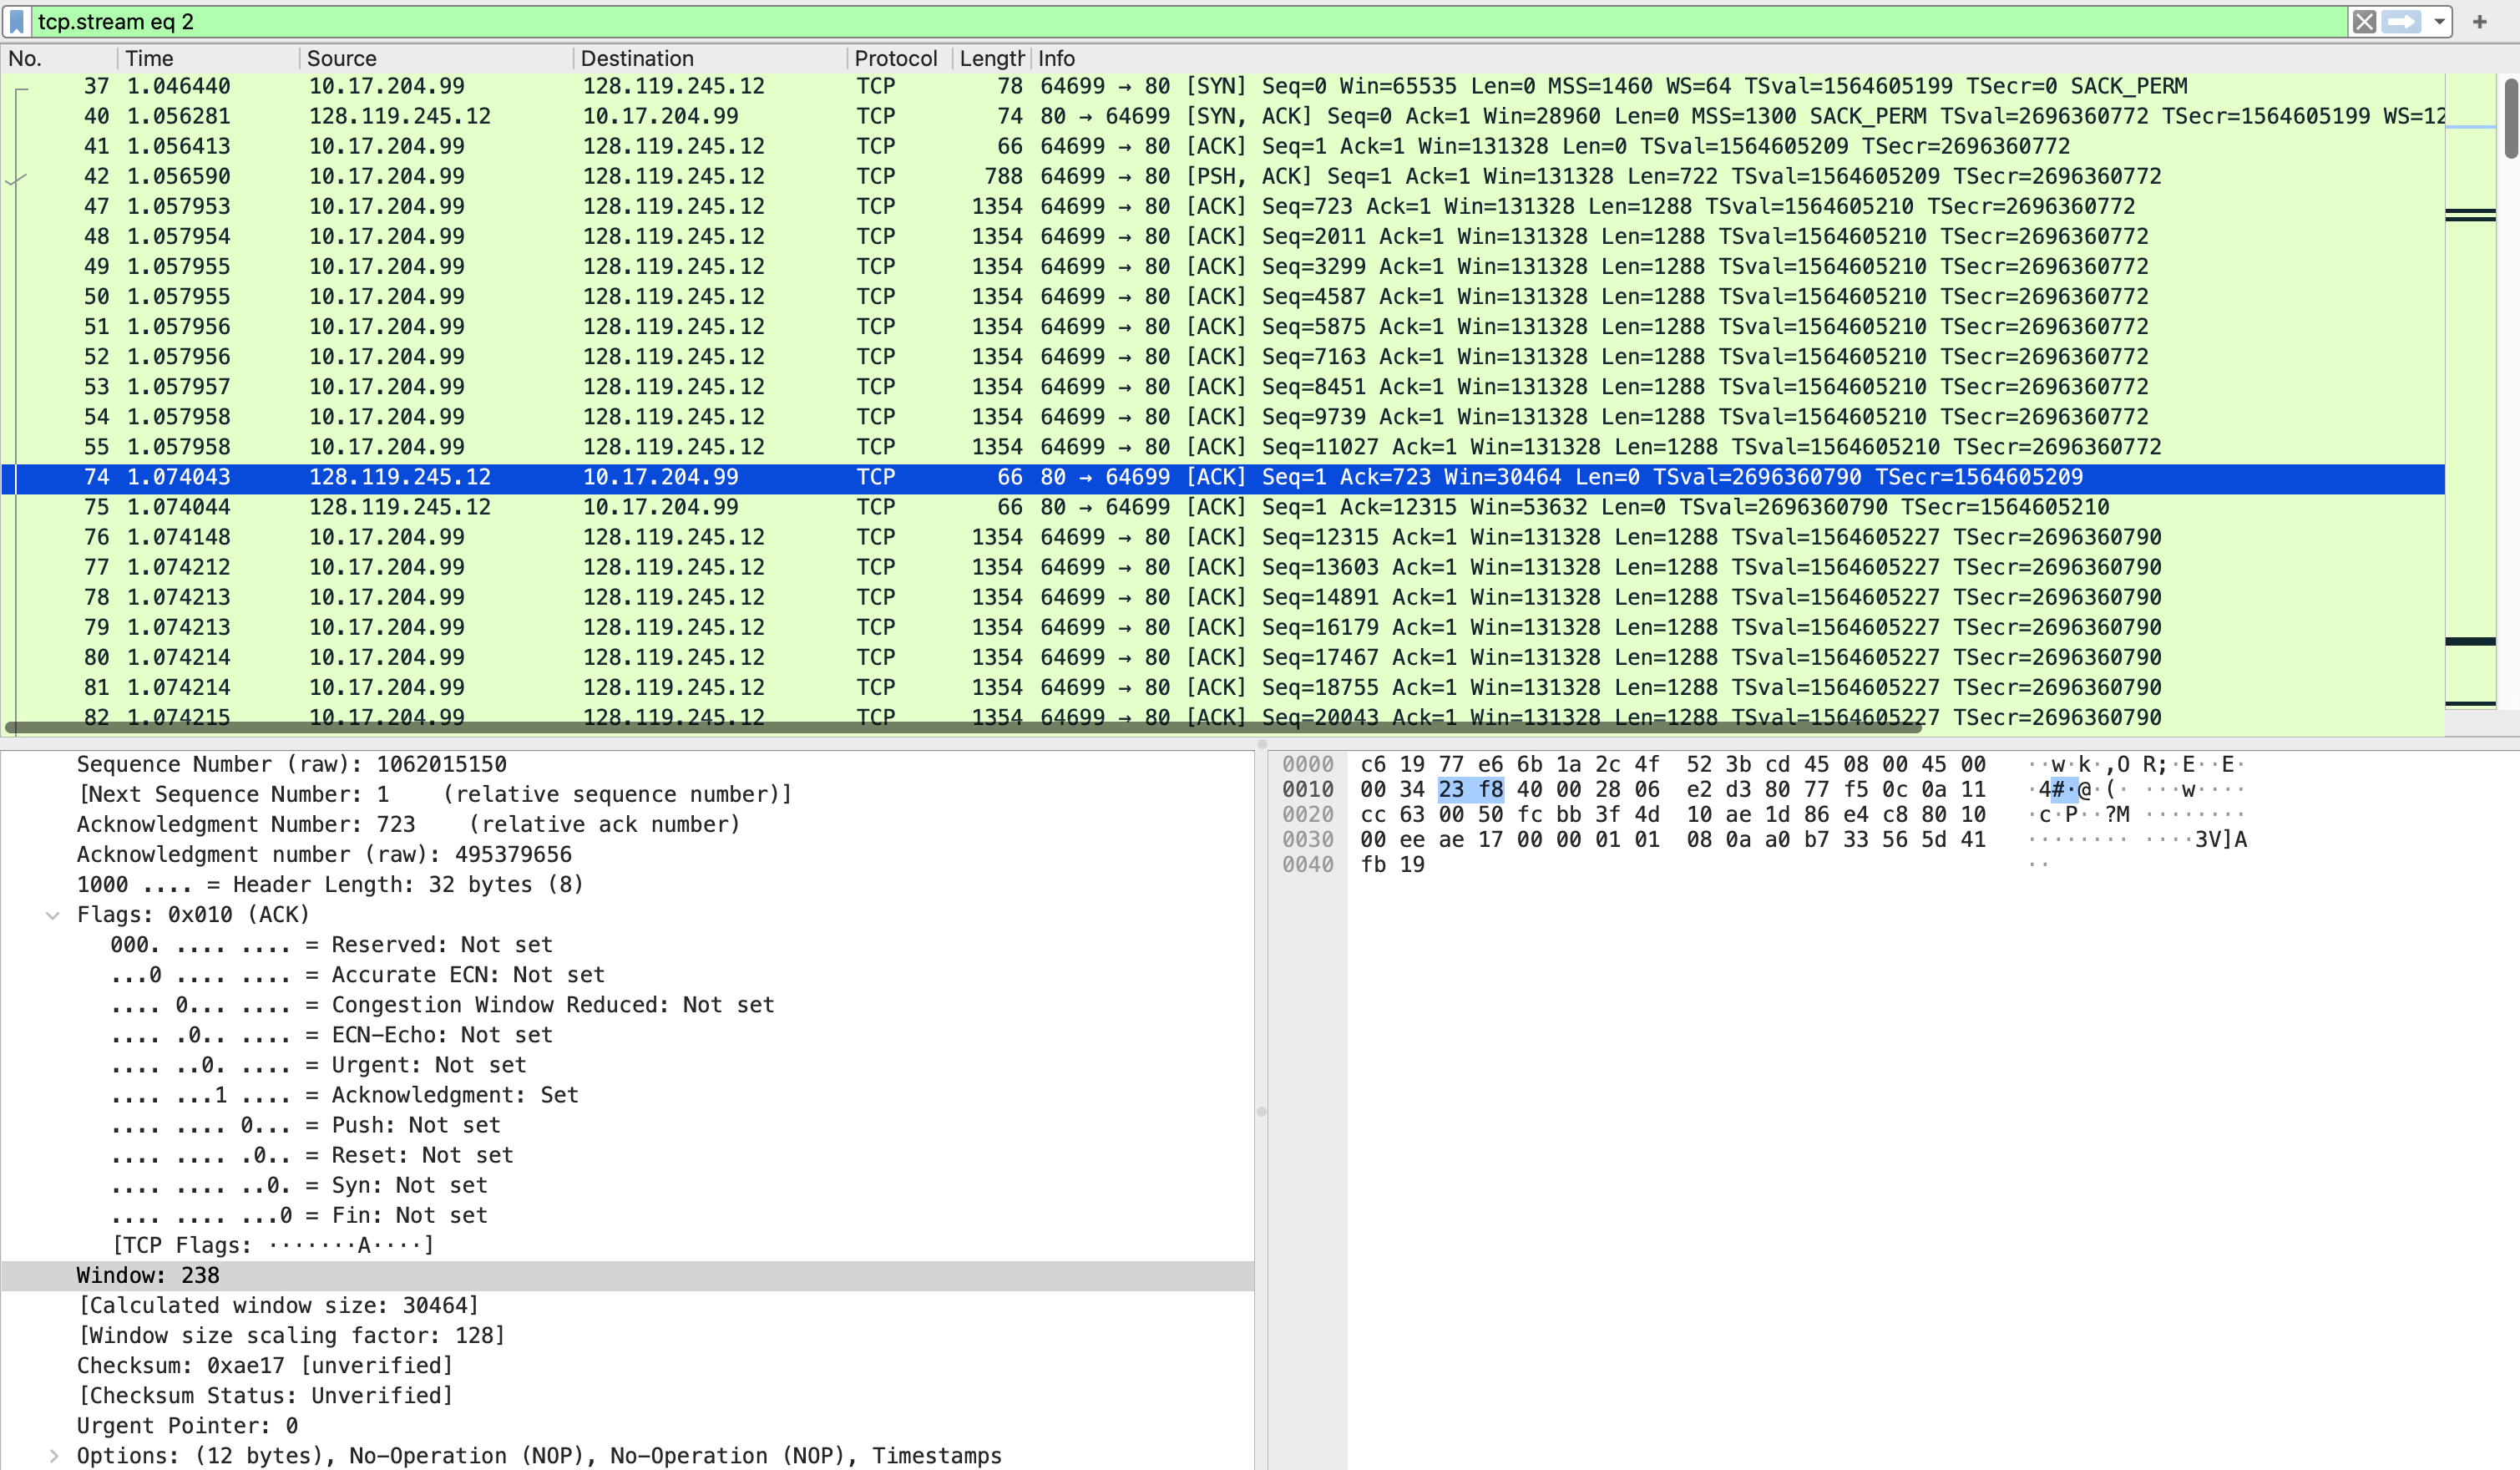
\includegraphics[width=0.8\textwidth]{9-1.png}
\end{figure}
\begin{figure}[H]
    \centering
    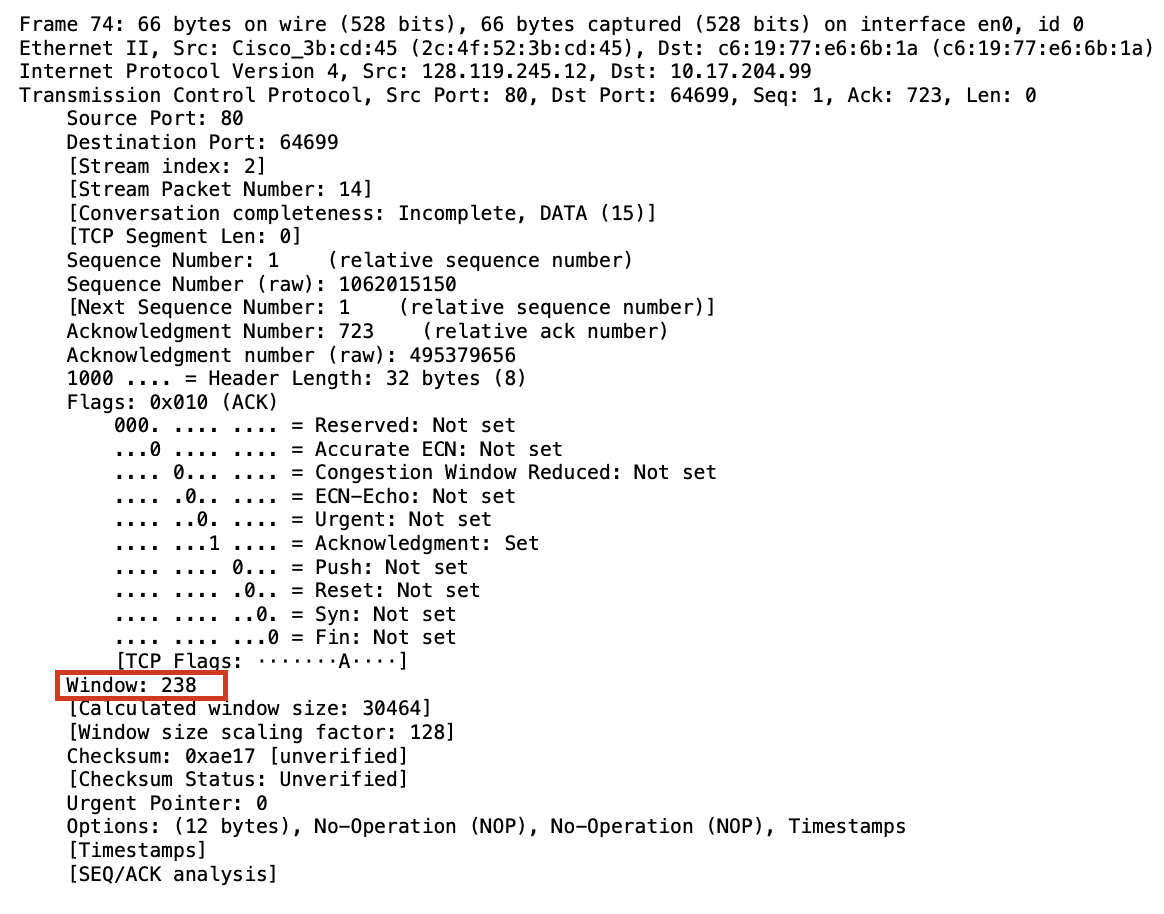
\includegraphics[width=0.8\textwidth]{9-2.png}
\end{figure}

\subsection{}
Yes, there are retransmitted segments in the trace.
I used a filter.
\begin{lstlisting}[language=bash]
    tcp.analysis.retransmission || tcp.analysis.fast_retransmission
\end{lstlisting}
Also in the "info" column, we can find the retransmitted segments.
\begin{figure}[H]
    \centering
    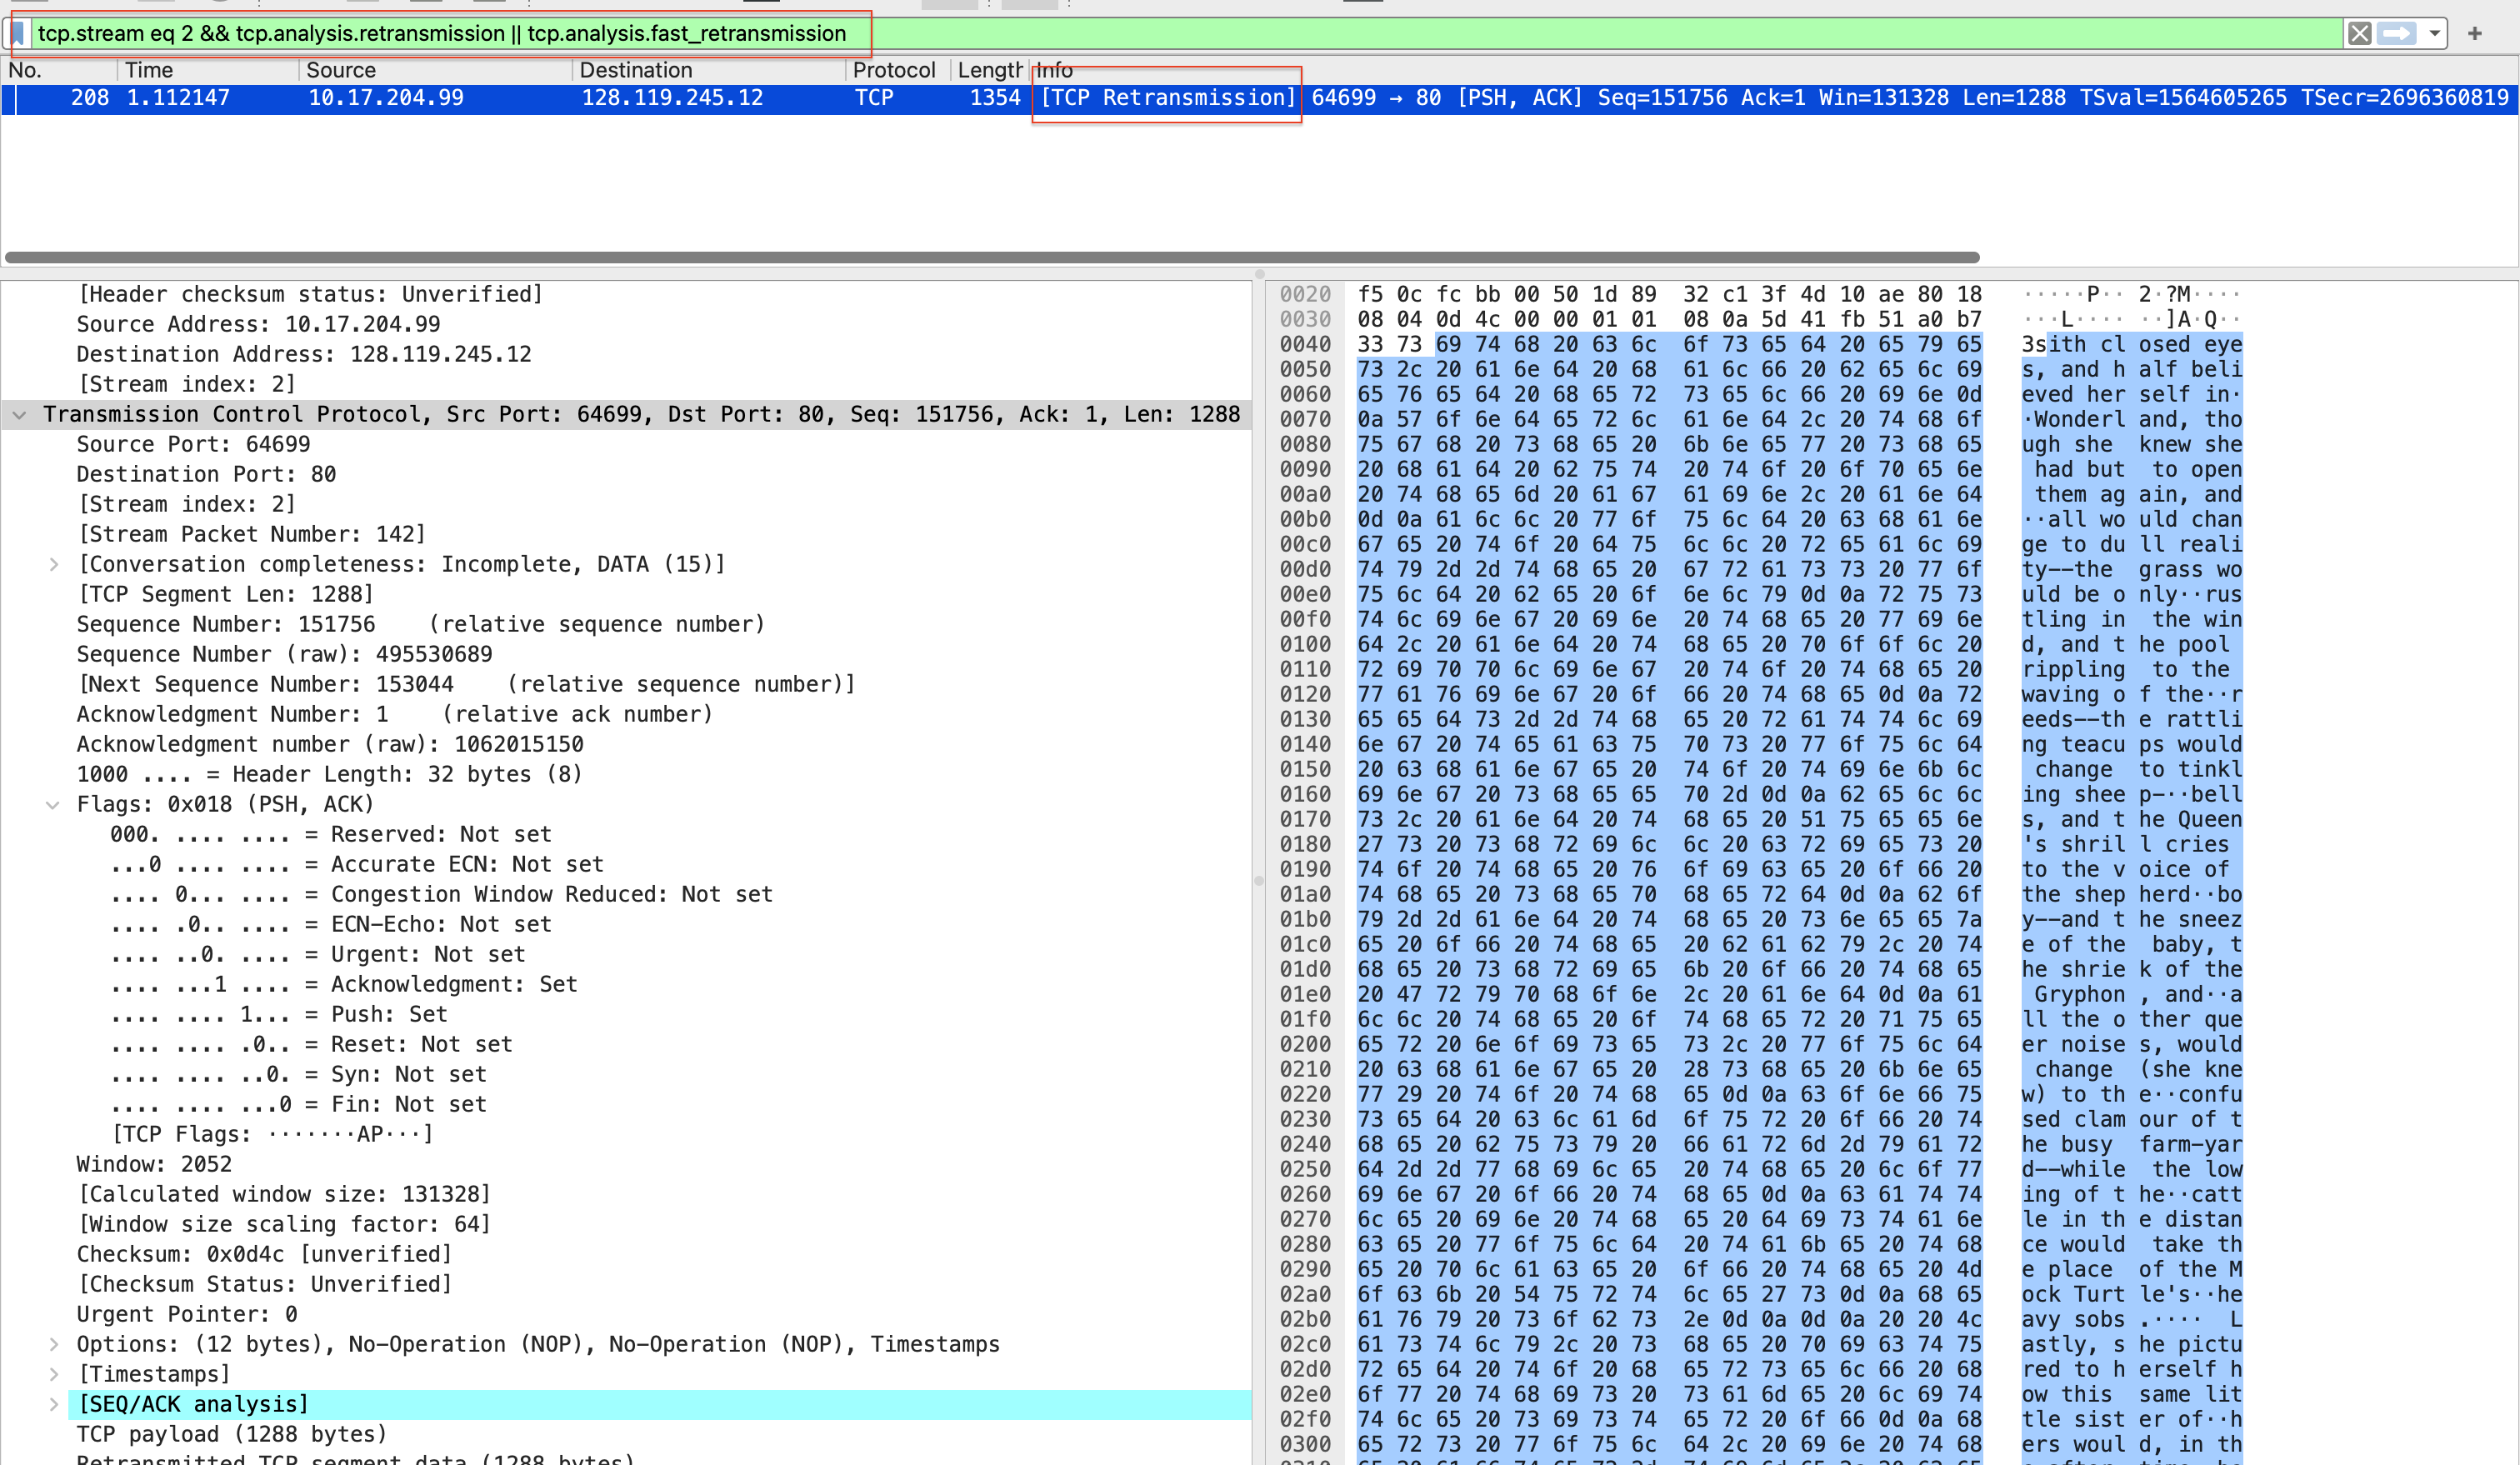
\includegraphics[width=0.7\textwidth]{10-1.png}
\end{figure}

\subsection{}
From the trace, each TCP segment has a length of 1288 bytes.
We can see from the screenshot below\\
Frame 47: Seq = 723, Len = 1288;\\
Frame 48: Seq = 2011, Len = 1288;\\
\begin{figure}[H]
    \centering
    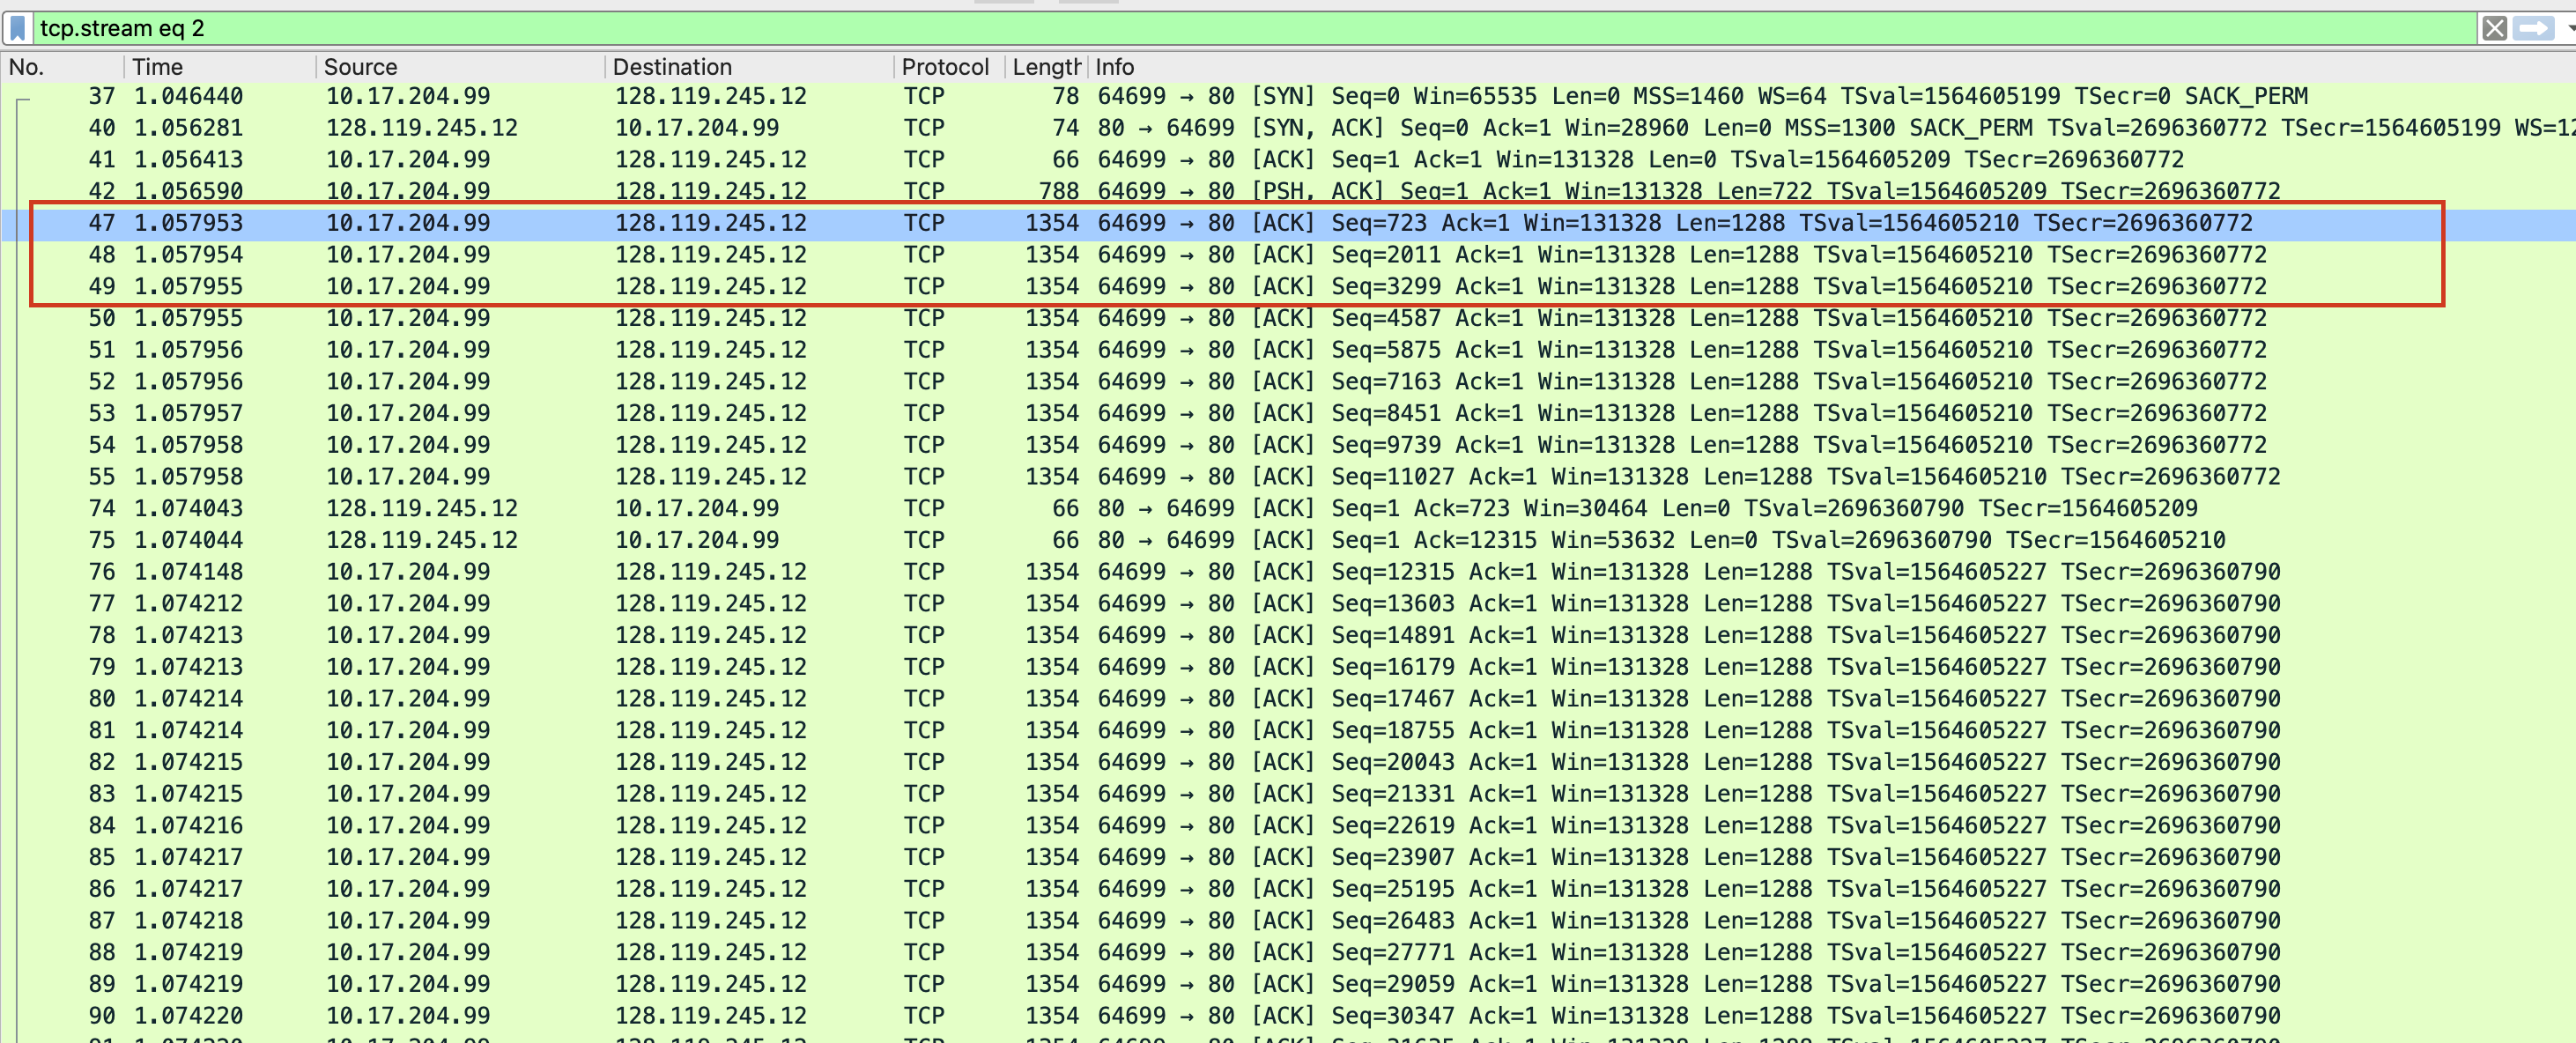
\includegraphics[width=0.8\textwidth]{11-1.png}
\end{figure}
I don't really find the receiver ACKing exactly every other segment,
but I can find that the receiver's delaying ACKing.
Between Packets 55 and 75:
The client sends multiple segments. The server sends Packet 75 (ACK=12315), skipping intermediate ACKs for segments like Packet 53 (Seq=8451) and Packet 54 (Seq=9739).
\begin{figure}[H]
    \centering
    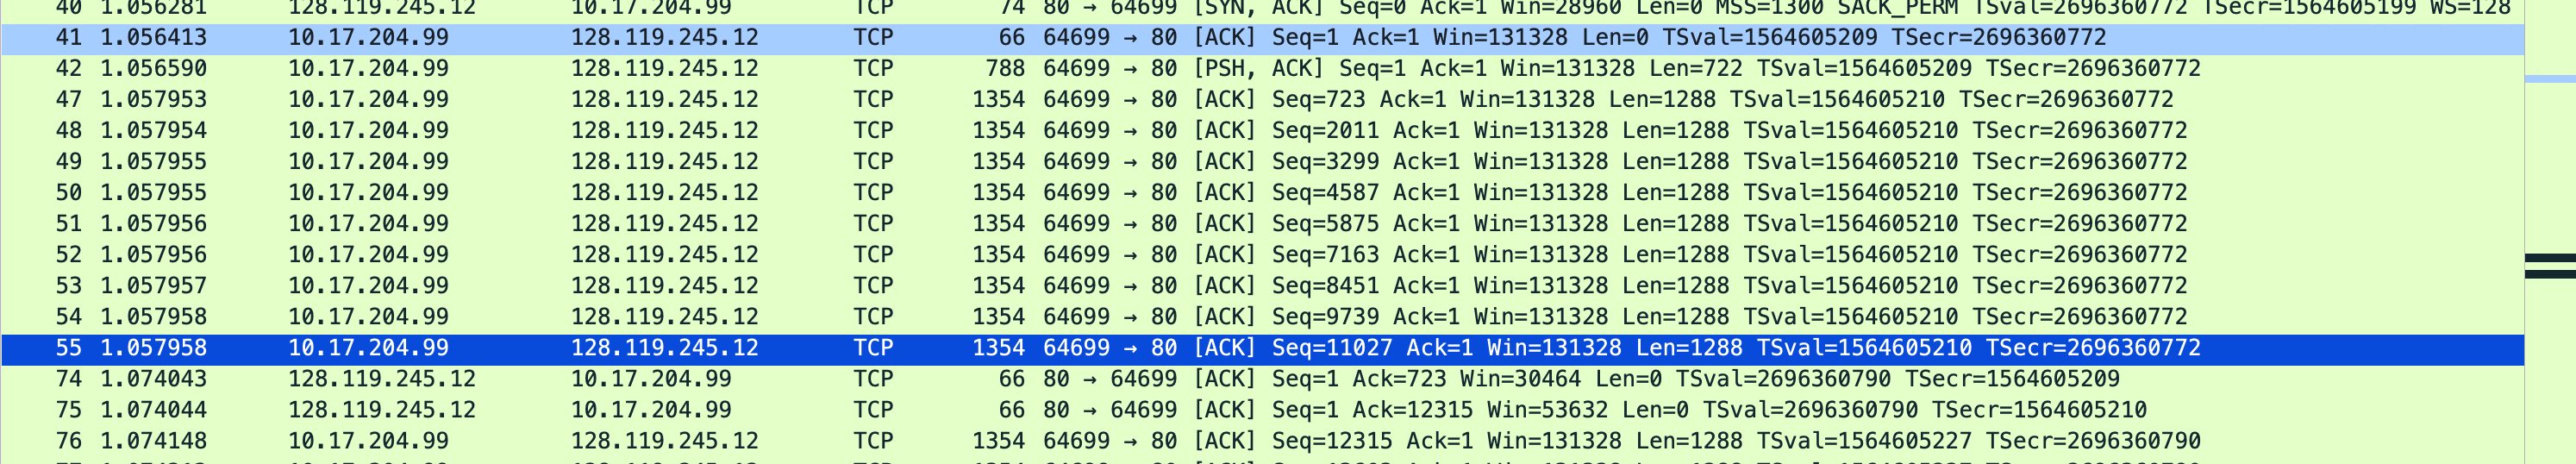
\includegraphics[width=0.8\textwidth]{11-2.png}
\end{figure}
\subsection{}
Total time: $T_{total} = T_{end} - T_{start} = 1.121956 - 1.046440 = 0.075516$ s.
\begin{figure}[H]
    \centering
    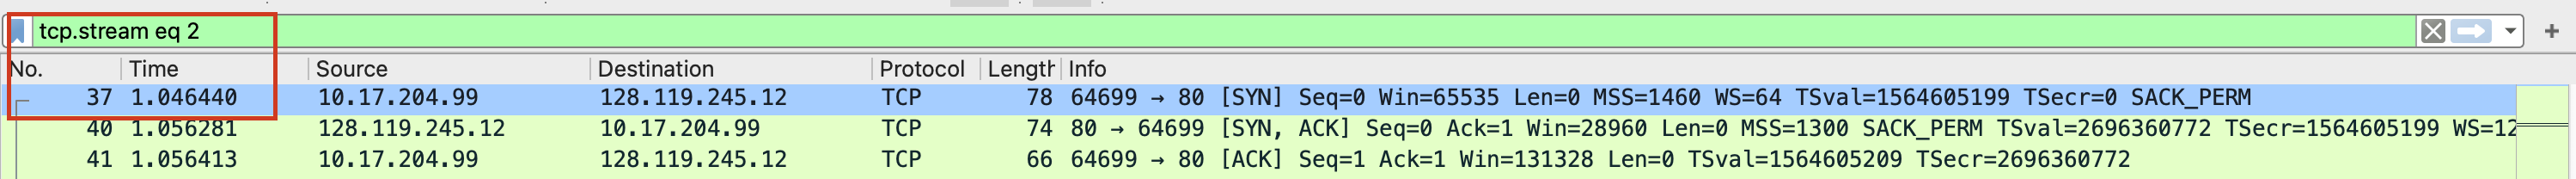
\includegraphics[width=0.8\textwidth]{12-1.png}
\end{figure}
\begin{figure}[H]
    \centering
    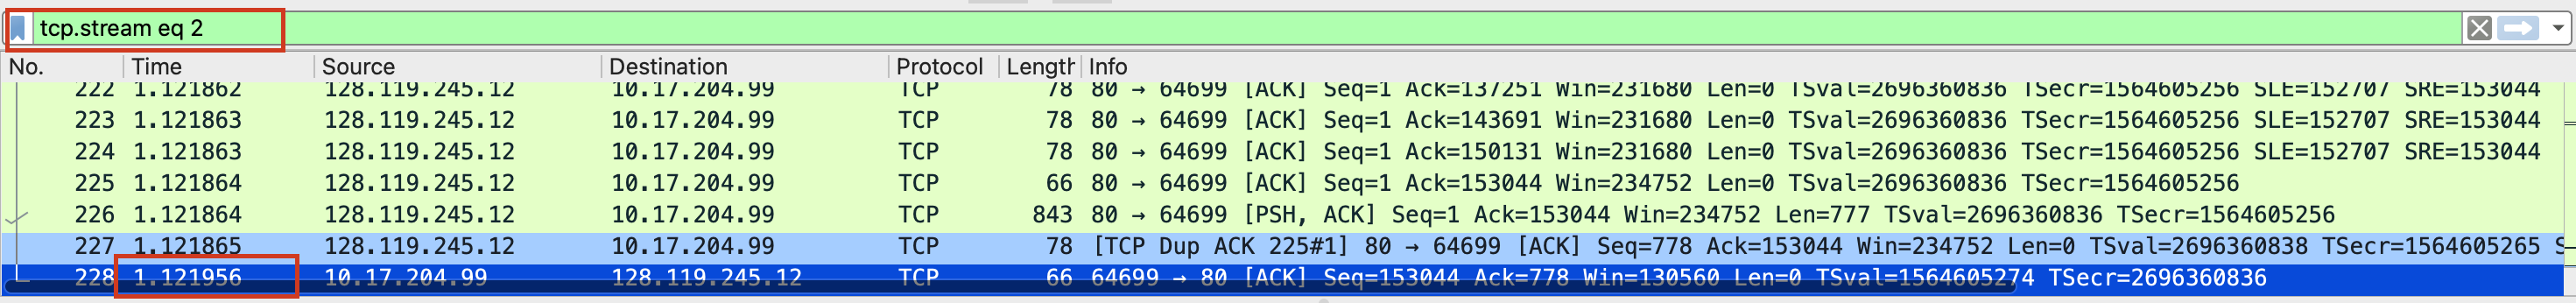
\includegraphics[width=0.8\textwidth]{12-2.png}
\end{figure}
And the final ack number is 153044. \\So
the throughput is \\$153044 \times 8 / 0.075516 = 16213146.9 = 16.21$ Mbps.

\section{TCP Congestion Control}

\subsection{}
As required, using the tcp-ethereal-trace-1 to answer the first questions.
The Slow start phase is around 0-0.2s(Marked by the red square), and the Congestion Avoidance phase is after 0.2s.
\begin{figure}[H]
    \centering
    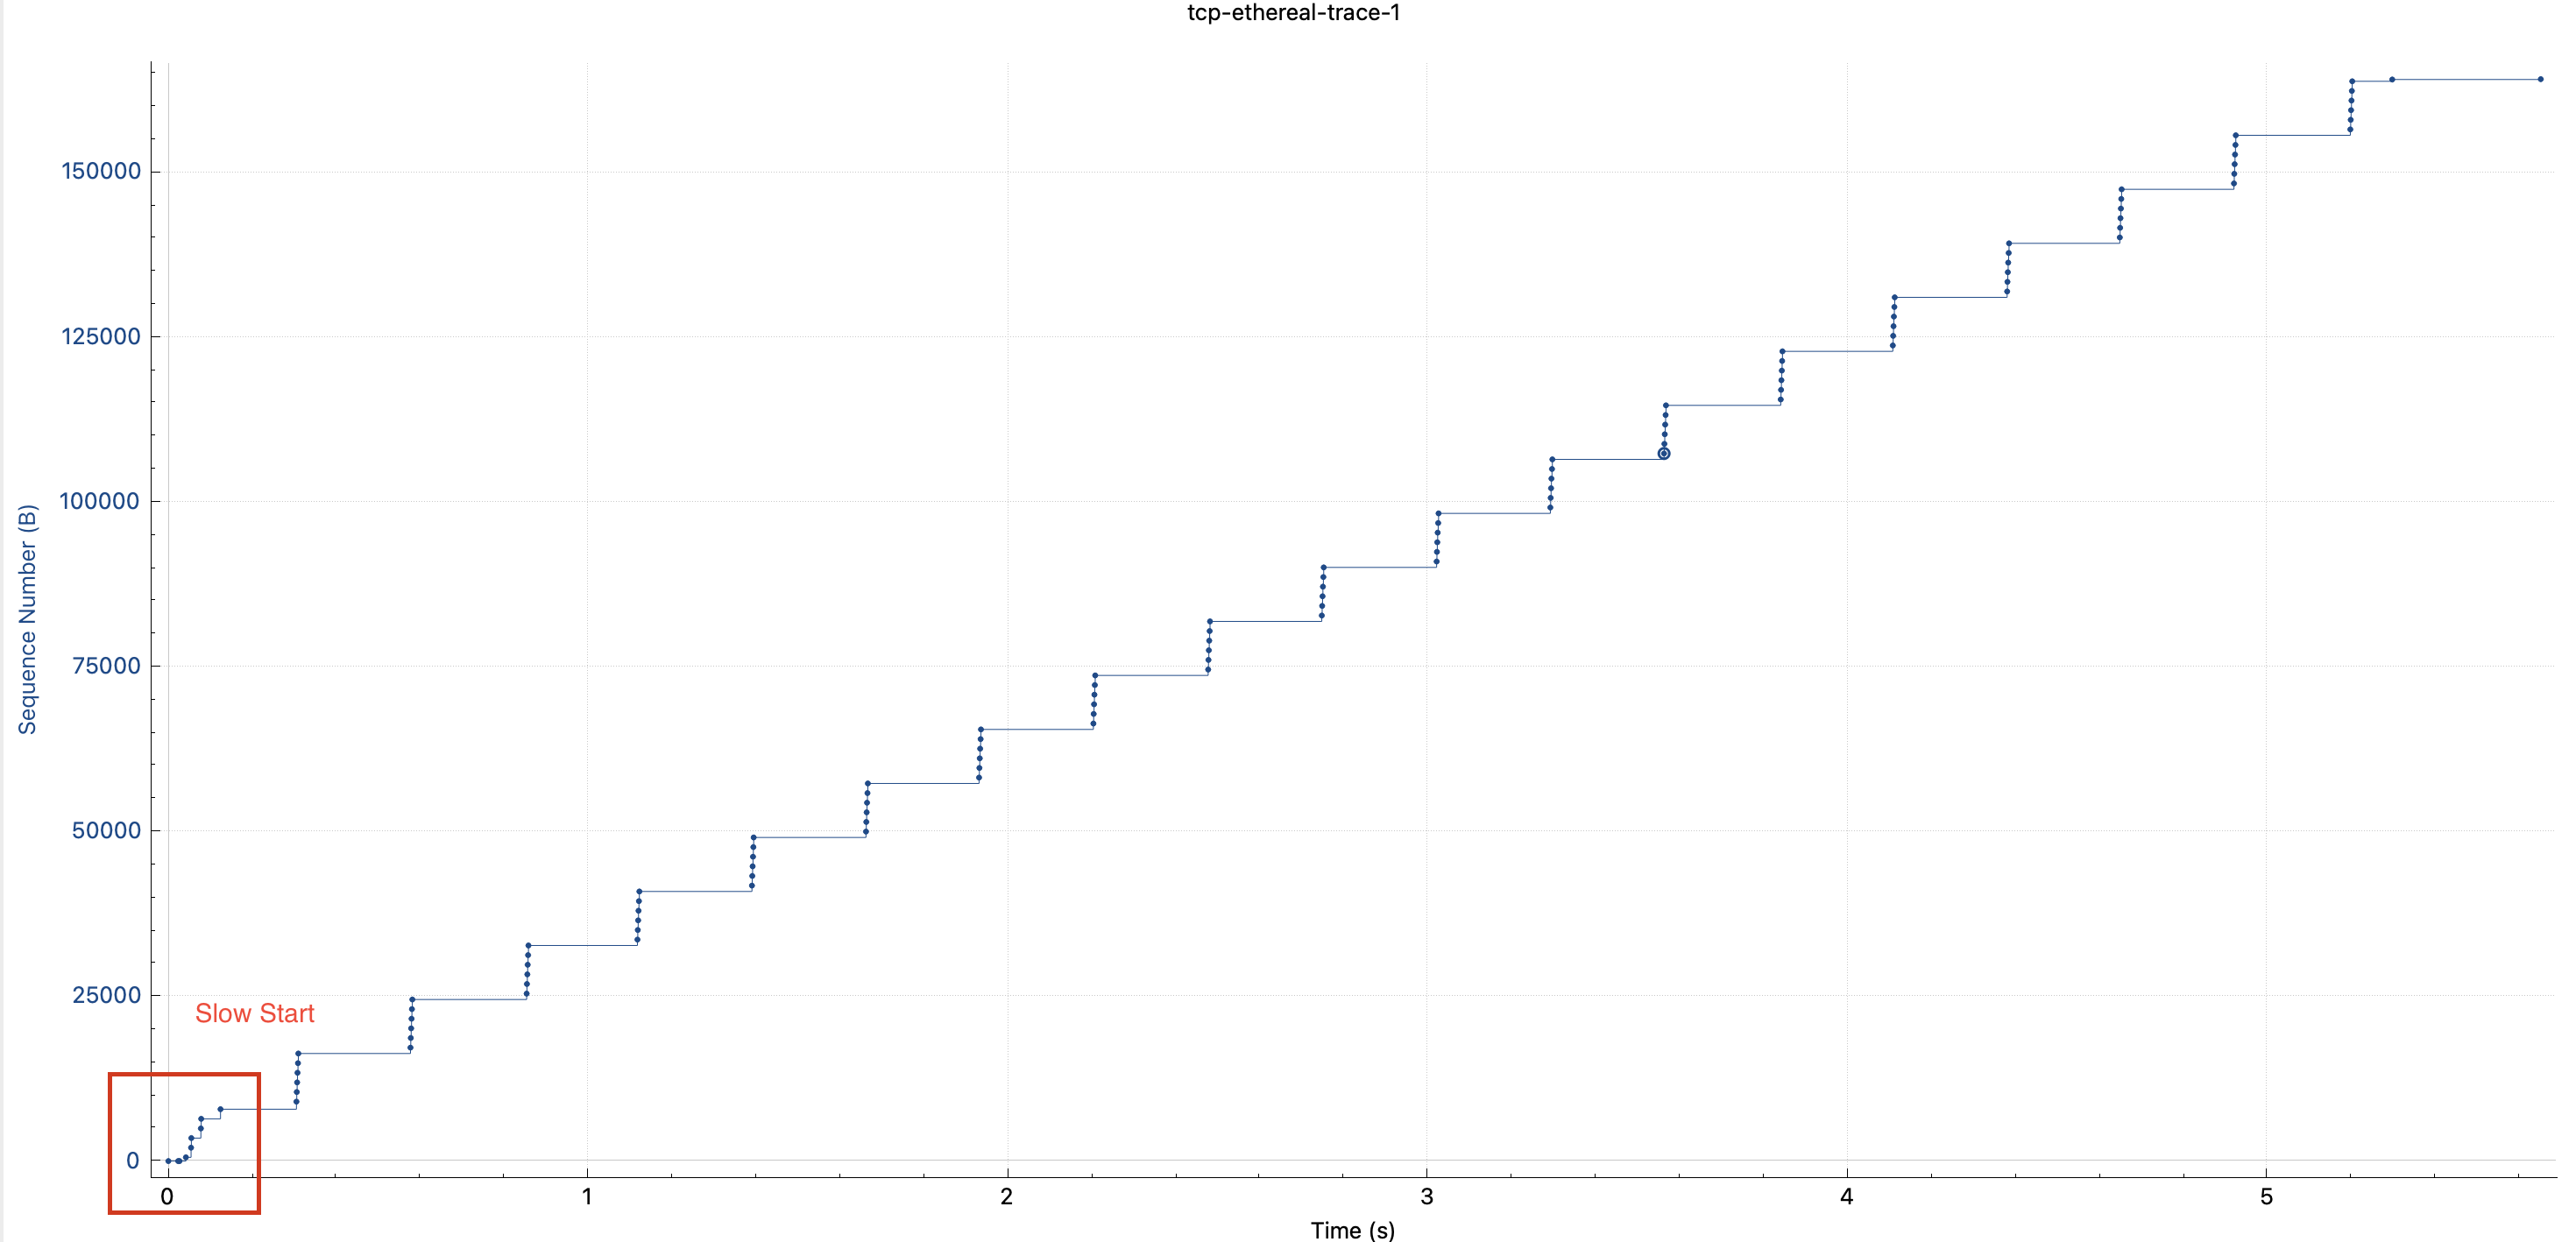
\includegraphics[width=0.8\textwidth]{13-1.png}
\end{figure}
What's different from the ideal case is that
sequence number increase remains smooth and linear
after the slow start phase and no
obvious packet loss like dramatic decrease, instead,
the sequence number increases with a smooth transition.

\subsection{}
Using my own trace to answer the second question.
The whole trace is in the slow start phase since the sequence number increases exponentially.
It is maybe because the data transfered is not large enough to trigger the congestion avoidance phase.
So there is nowhere to see the congestion avoidance phase.
\begin{figure}[H]
    \centering
    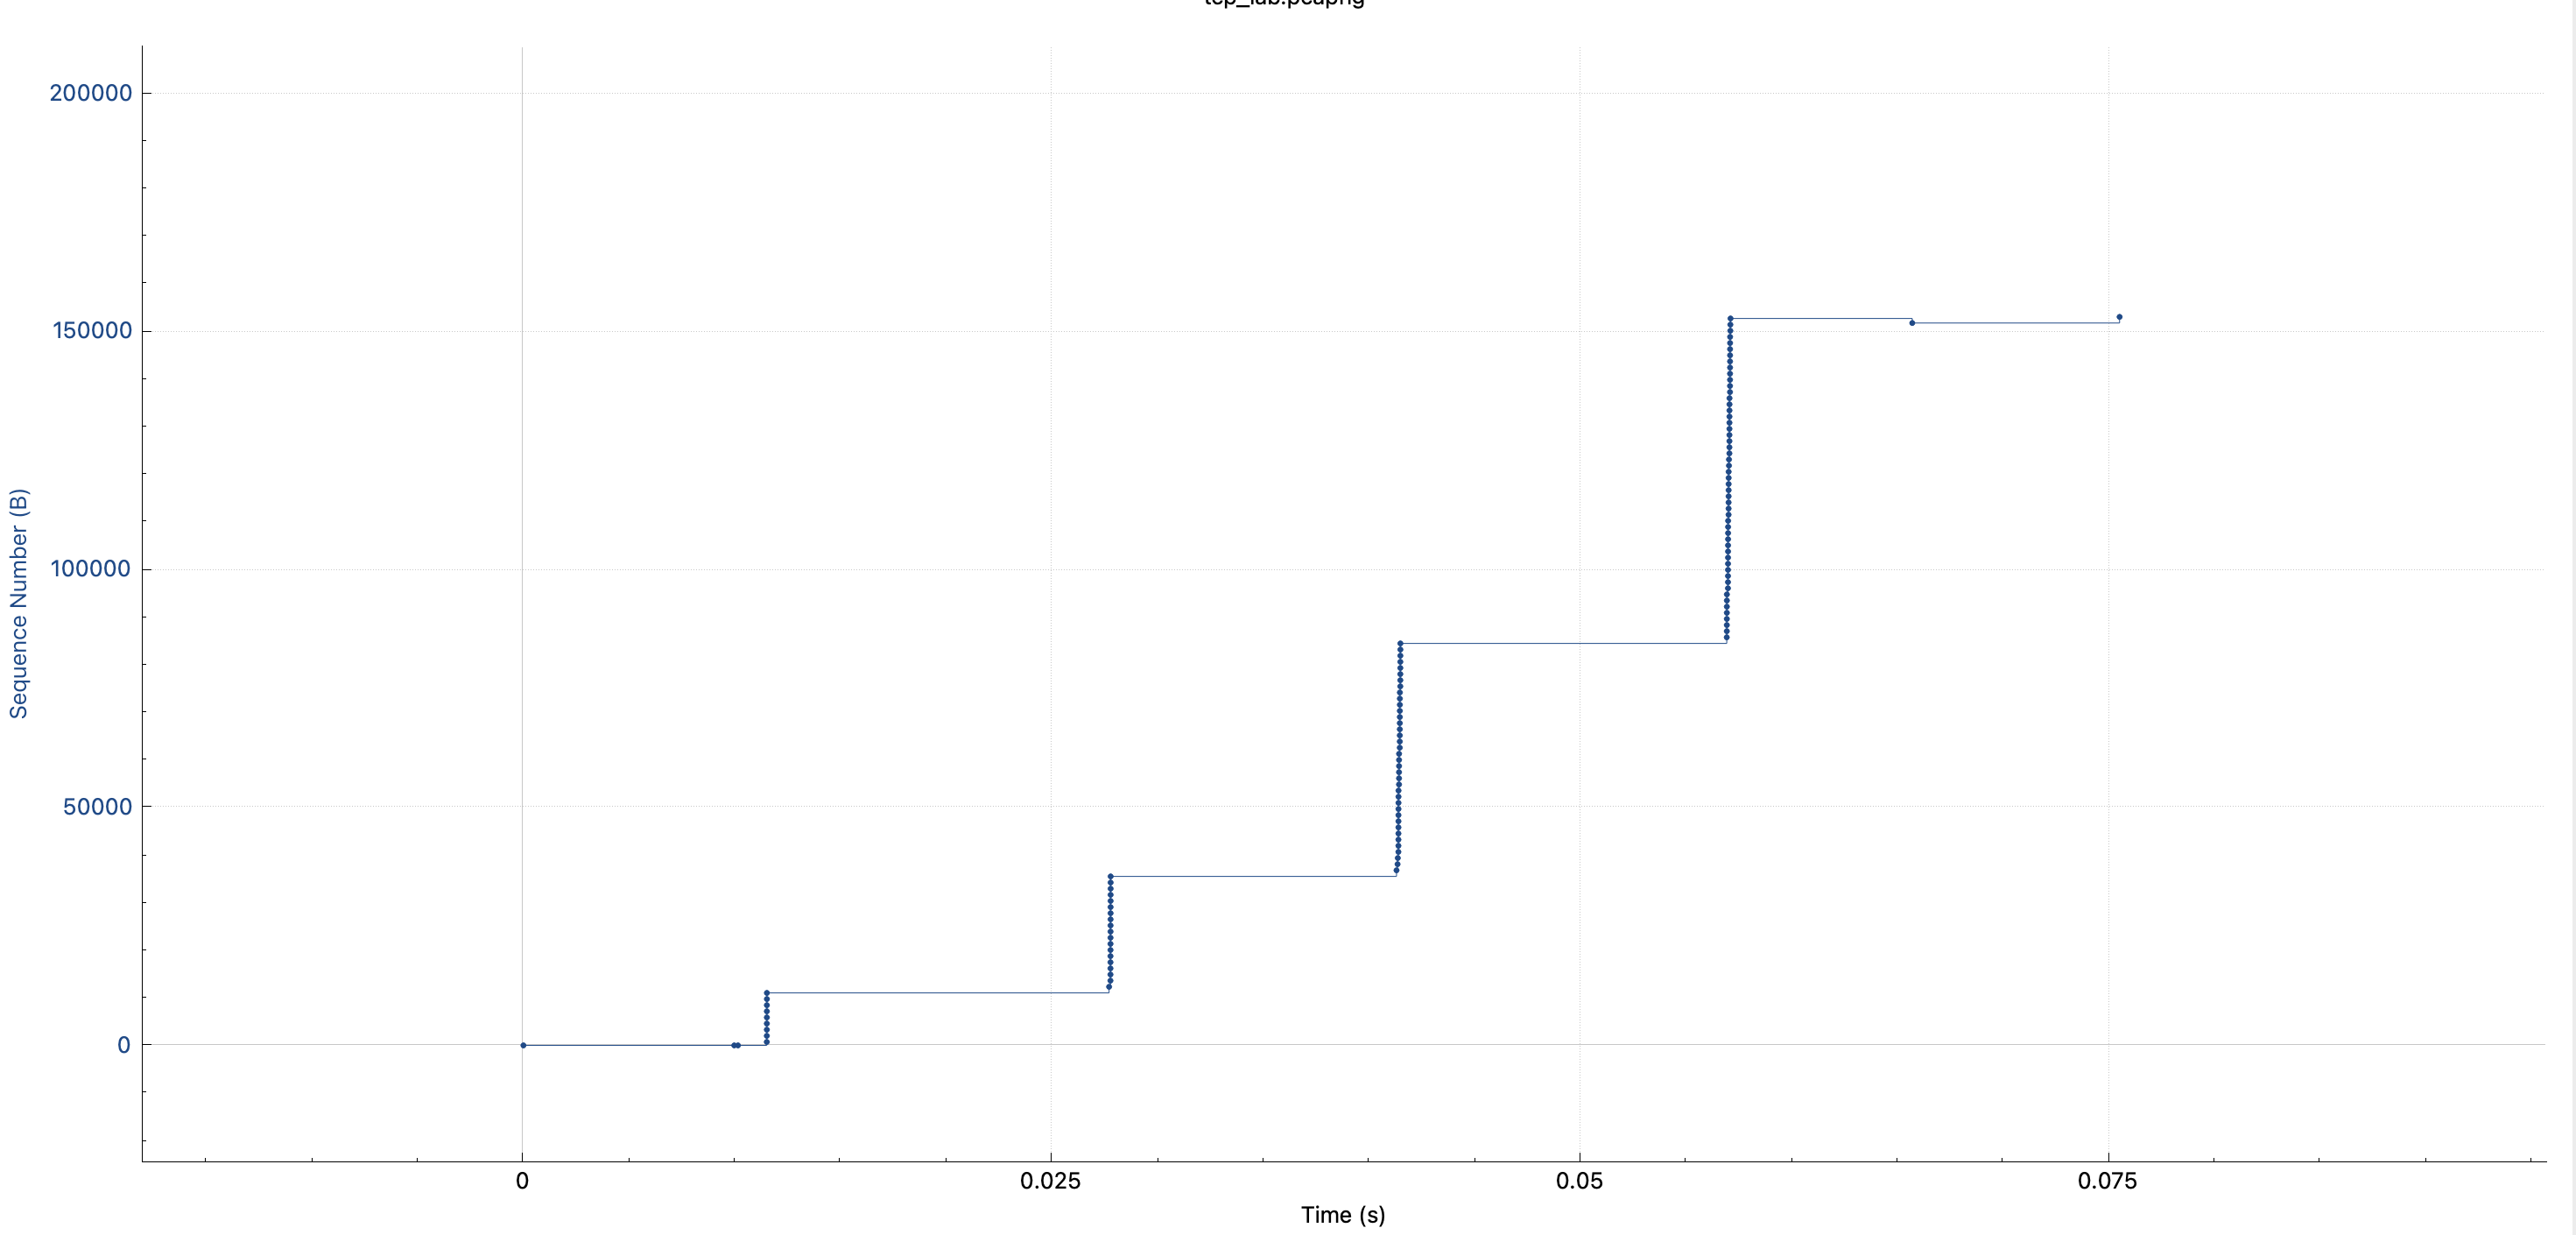
\includegraphics[width=0.8\textwidth]{14-1.png}
\end{figure}
As a result, it is hard to tell the difference between this graph and
the ideal case. However, it might because the initial congestion window here
is larger than the ideal case, which is also a possible reason and difference here.
\end{CJK*}
\end{document}
